% Options for packages loaded elsewhere
\PassOptionsToPackage{unicode}{hyperref}
\PassOptionsToPackage{hyphens}{url}
%
\documentclass[
  12pt,
]{article}
\usepackage{amsmath,amssymb}
\usepackage{lmodern}
\usepackage{ifxetex,ifluatex}
\ifnum 0\ifxetex 1\fi\ifluatex 1\fi=0 % if pdftex
  \usepackage[T1]{fontenc}
  \usepackage[utf8]{inputenc}
  \usepackage{textcomp} % provide euro and other symbols
\else % if luatex or xetex
  \usepackage{unicode-math}
  \defaultfontfeatures{Scale=MatchLowercase}
  \defaultfontfeatures[\rmfamily]{Ligatures=TeX,Scale=1}
  \setmainfont[]{Arial}
\fi
% Use upquote if available, for straight quotes in verbatim environments
\IfFileExists{upquote.sty}{\usepackage{upquote}}{}
\IfFileExists{microtype.sty}{% use microtype if available
  \usepackage[]{microtype}
  \UseMicrotypeSet[protrusion]{basicmath} % disable protrusion for tt fonts
}{}
\makeatletter
\@ifundefined{KOMAClassName}{% if non-KOMA class
  \IfFileExists{parskip.sty}{%
    \usepackage{parskip}
  }{% else
    \setlength{\parindent}{0pt}
    \setlength{\parskip}{6pt plus 2pt minus 1pt}}
}{% if KOMA class
  \KOMAoptions{parskip=half}}
\makeatother
\usepackage{xcolor}
\IfFileExists{xurl.sty}{\usepackage{xurl}}{} % add URL line breaks if available
\IfFileExists{bookmark.sty}{\usepackage{bookmark}}{\usepackage{hyperref}}
\hypersetup{
  pdftitle={Broadband connection and election in Brazil: what is role of the internet?},
  pdfauthor={Thiago Mendes Rosa},
  hidelinks,
  pdfcreator={LaTeX via pandoc}}
\urlstyle{same} % disable monospaced font for URLs
\usepackage[margin=1in]{geometry}
\usepackage{graphicx}
\makeatletter
\def\maxwidth{\ifdim\Gin@nat@width>\linewidth\linewidth\else\Gin@nat@width\fi}
\def\maxheight{\ifdim\Gin@nat@height>\textheight\textheight\else\Gin@nat@height\fi}
\makeatother
% Scale images if necessary, so that they will not overflow the page
% margins by default, and it is still possible to overwrite the defaults
% using explicit options in \includegraphics[width, height, ...]{}
\setkeys{Gin}{width=\maxwidth,height=\maxheight,keepaspectratio}
% Set default figure placement to htbp
\makeatletter
\def\fps@figure{htbp}
\makeatother
\setlength{\emergencystretch}{3em} % prevent overfull lines
\providecommand{\tightlist}{%
  \setlength{\itemsep}{0pt}\setlength{\parskip}{0pt}}
\setcounter{secnumdepth}{5}
\setlength\parindent{24pt}
\setlength{\textfloatsep}{0.5cm}
\setlength{\floatsep}{0.5cm}
\usepackage[bottom]{footmisc}
\usepackage{indentfirst}
\usepackage{datetime}
\usepackage{setspace}
\onehalfspace
\usepackage{pdfpages}
\usepackage{floatrow}
\usepackage{amsmath}
\usepackage{bbm}
\usepackage{morefloats}
\usepackage{pbox}
\usepackage{graphicx}
\usepackage{tikz}
\usepackage{booktabs}
\usepackage{xcolor}
\usepackage{tabularx}
\floatplacement{figure}{H}
\floatsetup[figure]{capposition=top}
\floatsetup[table]{capposition=top}
\usepackage[bf]{caption}
\captionsetup{justification=raggedright,singlelinecheck=false}
\captionsetup[table]{belowskip=0pt}
\usepackage{placeins}
\usepackage{rotating}
\usepackage[hyphenbreaks]{breakurl}
\usepackage{pdflscape}
\usepackage{sectsty} \allsectionsfont{\centering}
\usepackage{tabu}
\usepackage{longtable}
\usepackage{threeparttable}
\usepackage[normalem]{ulem}
\usepackage{makecell}
\usepackage{multirow}
\usepackage{afterpage}
\ifluatex
  \usepackage{selnolig}  % disable illegal ligatures
\fi
\newlength{\cslhangindent}
\setlength{\cslhangindent}{1.5em}
\newlength{\csllabelwidth}
\setlength{\csllabelwidth}{3em}
\newenvironment{CSLReferences}[2] % #1 hanging-ident, #2 entry spacing
 {% don't indent paragraphs
  \setlength{\parindent}{0pt}
  % turn on hanging indent if param 1 is 1
  \ifodd #1 \everypar{\setlength{\hangindent}{\cslhangindent}}\ignorespaces\fi
  % set entry spacing
  \ifnum #2 > 0
  \setlength{\parskip}{#2\baselineskip}
  \fi
 }%
 {}
\usepackage{calc}
\newcommand{\CSLBlock}[1]{#1\hfill\break}
\newcommand{\CSLLeftMargin}[1]{\parbox[t]{\csllabelwidth}{#1}}
\newcommand{\CSLRightInline}[1]{\parbox[t]{\linewidth - \csllabelwidth}{#1}\break}
\newcommand{\CSLIndent}[1]{\hspace{\cslhangindent}#1}

\title{Broadband connection and election in Brazil: what is role of the
internet?}
\author{Thiago Mendes Rosa\footnote{Universidade de Brasília,
  \href{mailto:thiagomendesrosa@outlook.com}{\nolinkurl{thiagomendesrosa@outlook.com}}}}
\date{2021-04-11}

\begin{document}
\maketitle

\let\oldthebibliography\thebibliography
\let\endoldthebibliography\endthebibliography
\renewenvironment{thebibliography}[1]{
  \begin{oldthebibliography}{#1}
    \setlength{\itemsep}{0em}
    \setlength{\parskip}{0em}
}
{
  \end{oldthebibliography}
}

\allsectionsfont{\centering}

\hypertarget{abstract}{%
\section*{Abstract}\label{abstract}}
\addcontentsline{toc}{section}{Abstract}

We investigate the relationship between broadband internet velocity and
election outcomes in Brazil (2008, 2010 and 2012). Using a robust
identification strategy, a RDD applied to the roll out of Backhaul
program, we explore jumps in internet velocity according to population
size as identification strategy. Results indicate no relationship
between internet speed and political outcomes -- turnout, blank and null
percentage votes, left parties vote share, small party or young
candidate vote share and campaign budget. Our findings diverge from some
positive/negative results reported before, usually applied to
democracies with institutional backgrounds distinct of the one observed
in Brazil, suggesting that the relationship between internet and
electoral outcomes does not apply everywhere.

\textbf{Keywords:} Internet, RDD, elections.

\allsectionsfont{\raggedright}

\clearpage

\hypertarget{introduction}{%
\section*{Introduction}\label{introduction}}
\addcontentsline{toc}{section}{Introduction}

The aim of this paper is to asses the impact of broadband internet
velocity on political outcomes: turnout, vote share, types of votes and
campaign budget.

The way how people get informed about politics has changed dramatically
over the years (Bimber 2003). If in XIX century newspaper was the main
source of information, in the beginning of XX's radio took its place,
surpassed by television in the middle of the same century. Today, a new
type of media seems to be taking the lead: the internet.

Although the world wide web is an almost 30 years-old technology,
broadband connection is an even recent event (Maddux \& Johnson 1997).
Internet velocity capable of streaming videos became popular just in the
XXI century. Social networks, like Facebook, YouTube and Twitter are
relatively infant phenomenons\footnote{Facebook was launched in 2004,
  YouTube in 2005 and Twitter in 2006.}, becoming popular globally only
in the late of 2000's. Mobile broadband connections, thanks to 3G
technology (followed by 4G) and massification of smartphones\footnote{The
  first Iphone was launched in 2007.}, helped internet to reach a
greater number of users. New social medias, like WhatsApp, Instagram and
Telegram are now everyday tools\footnote{WhatsApp was launched in 2009,
  Instagram in 2010 and Telegram in 2013.}, with popularity increasing
in an exponential fashion, being common even for business. A new wave,
with 5G technology and the ``internet of things'' is coming to continue
the revolution begun in the past century, with connections speed and
quality increasing every day, with new possibilities of business.

Thus, information dissemination gained range and speed, reaching more
people, almost instantaneously, nearly in any part of the world.
Geographic barriers were broken and the amount of information are vast.
Before these new possibilities, a question arises: how this new scenario
affects social interaction? Furthermore, how do people are doing
politics in this new environment? In particular, if people have tools to
be more informed, do they increase their participation in elections?
Could vote preferences change with introduction of this new technology?
Or, on contrary, have this new possibilities of entertainment deviate
people from political discussion? Is it possible that internet did not
change politics at all?

These questions are not easy to be answered for several reasons.
Availability of internet is not random and characteristics like income,
schooling and geographic conditions may determine if an internet service
provider will be accessible for individuals (Falck \emph{et al.} 2014;
Miner 2015; Campante \emph{et al.} 2017). Also, institutional and
political backgrounds may possible influence internet-political
relationship.

This is not a novel issue. Relationship between internet and politics
has been focus of study in several fields (Bimber 1998; Larson 2004;
Czernich 2012; Jaber 2013; Falck \emph{et al.} 2014; Gavazza \emph{et
al.} 2015; Poy \& Schüller 2016; Campante \emph{et al.} 2017), and this
paper aims to contribute with this literature, studying internet
velocity impacts on politics in Brazil. Focusing on a single country, we
have best tools to control for possible confounders, and taking
advantage of a specific rule for broadband roll out, where number of
inhabitants determines the internet velocity of municipalities (the
backhaul program), we have a robust identification strategy, which
creates an ideal instrument to deal with internet velocity endogeneity.
Following Cattaneo \emph{et al.} (2018), we use multiple cumulative
cutoffs design to estimate effects.

In the most recent Brazilian presidential election, internet had a major
role in result. In 2018, Mr.~Bolsonaro, with a little fraction of
financial resources used by his opponents\footnote{While Mr.~Bolsonaro
  expended R\$ 2.46 million in his campaign, the second place,
  Mr.~Haddad, expended R\$ 37.5 million, a figure 15 times higher.
  Complete figures are available in
  \url{http://divulgacandcontas.tse.jus.br/}.} and with only eight
seconds of national advertising time in television\footnote{\url{https://agenciabrasil.ebc.com.br/politica/noticia/2018-08/tse-apresenta-tempos-de-radio-e-tv-de-presidenciaveis}},
managed to go to the second round of presidential elections, with
46.03\% of votes, and won elections with a 10 p.p. margin difference.
According to Brazilian newspapers, the strength of Mr.~Bolsonaro in the
social medias was capital to his victory\footnote{\url{https://www.correiobraziliense.com.br/app/noticia/politica/2018/10/28/interna_politica,715584/bolsonaro-fez-das-redes-sociais-o-caminho-certo-para-uma-provavel-vito.shtml},
  \url{https://g1.globo.com/politica/blog/cristiana-lobo/post/2018/12/31/redes-sociais-mudam-completamente-a-relacao-dos-eleitores-com-seus-representantes.ghtml},
  \url{https://noticias.uol.com.br/politica/eleicoes/2018/noticias/2018/10/09/como-midias-sociais-e-orcamentos-enxutos-derrubaram-cinco-mitos-eleitorais.htm}},
which makes Brazil an interesting case of study regarding the
relationship between internet and elections.

We go back a little in time and study if the beginning of broadband
internet played a role in election outcomes. Results suggests that, in
general, broadband internet speed is not related to political outcome in
Brazil. It seems that internet velocity did not influence turnout, blank
or null percentage votes, left parties vote share, the number of
candidates, a small party and young candidates vote share and campaign
budget, in 2008, 2010 and 2012 elections, which covers a national and
two local suffrage. The offices considered (president, mayor, deputies
or local legislators) did not make difference in results. These finds
are different from previous results reported in the literature, meaning
that institutional background or local idiosyncrasies may play an
important role in studies relating politics and internet. Positive and
negative relationship are reported for Germany, Italy and United Kingdom
(Falck \emph{et al.} 2014; Gavazza \emph{et al.} 2015; Campante \emph{et
al.} 2017), all of them with distinct political institutional background
compared with Brazilian's.

This paper is organized as follows: the first section presents the
theoretical framework linking internet to political outcomes, while the
next one reports the previous findings regarding its application. The
third section reviews the Brazilian institutional political background,
followed by the section with empirical strategy, data bases and
descriptive statistics. The fifth section presents our results, with a
final discussion in the sixth and last section.

\hypertarget{theoretical-framework}{%
\section{Theoretical framework}\label{theoretical-framework}}

There are some theories looking to explain why people vote (Downs 1957;
Riker \& Ordeshook 1968; Ferejohn \& Fiorina 1974; Uhlaner 1989; Aldrich
1993). One approach is to treat as a microeconomic problem in the
following way. In elections, individuals' problem is to choose the best
candidate(s) according to their preferences. But, there is an asymmetry
of information: there are many candidates (not considering uncontested
elections), and voters are not fully informed about their abilities.
Acquire information about them is costly, since they have to spend
resources to consume information (e.g.~from television, radio,
newspaper, internet or another people), that may include money and time.
Show up to cast the ballot also requires resources (transportation and
time, for example). More accurate decision requires more information,
which demands more resources, i.e.~is more costly. So, it can be viewed
as a maximization problem from the microeconomics point of view, which
can be solved by equalizing marginal costs and benefits. Benefits can be
viewed as the policies the most preferred candidate will conduct, a
civil duty or being party of the democratic process (Ali \& Lin 2013).

This problem changes over time with entrance of new technologies
(Gentzkow 2006). For example, when radio, television and internet were
not available, there were fewer options to people get informed about
candidates. Also, there were available less leisure alternatives. With
emergence of radio, then television and, finally, internet, these costs
and substitution effects may have changed. A first natural question that
someone could ask is: did these new technologies affect the decision of
voters? For newspaper, Gerber \emph{et al.} (2009), Gentzkow \emph{et
al.} (2011) and Drago \emph{et al.} (2014) report effects on elections
participation. According to Strömberg (2004) and Horacio \& Monteiro
(2014), radio affects people perception about politics, while DellaVigna
\& Kaplan (2007), Enikolopov \emph{et al.} (2011), Durante \& Knight
(2012), Gentzkow (2006) and Oberholzer-Gee \& Waldfogel (2009) shows the
impact of television (through news) on elections results.

How about the internet? Relationship between internet and politics has
been investigated since the end of 1990's (Bimber 1998). The effect on
information acquisition may be ambiguous depending on the hypothesis
used: if internet makes available new possibilities of entertainment,
people may substitute the time spent learning about politics with these
new type of leisure; on the other hand, if internet bring to people new
sources of politics information and channels of discussion, people may
be pushed toward politics. Finally, the cost and the time needed to find
candidates information or to find new possibilities of entertainment may
have changed relative prices. Once someone has access to internet, it is
possible to consume a variety of information with, in general, no
additional cost. The same is valid to leisure. A last possibility is
that the only thing substituted is the technology used to consume
information and leisure, making no difference in resources allocation at
all\footnote{If there is no, or little, consumption of politics
  information with an older technology, it might be the case that, even
  with a new technology, there is no preference for this type of
  information, resulting in no, or limited, shifting in its demand.}.

These changes may also take time to happen. Many types of media on
internet depends on broadband connection (like video streaming), only
available to the large public in the beginning of the XXI century.
Moreover, all content we have today were not available with the launch
of the internet. The same was true for television, where the diversity
of programs and shows existing today took time to be developed and
aired. Emergency of new technologies and its spread also affects
relative prices both for information and leisure over time with this
development.

While newspaper, radio and TV content production are more restricted and
with barrier entries, internet have opened doors to virtually anyone
produce information and media, interact with people and organize groups
of common interest, everything at a lower cost and time. Thus, it is
likely to exist a shift both in the demand and supply of information and
entertainment with internet arrival. It can potentially alter the manner
of how politics are made, since, with internet, politicians can reach
more people, quickly and at lower costs when compared with other medias.

One situation this new scenario brings is the social media consumption
of ``fake news''\footnote{Fake news is a popular term to define, in
  general, the spread of misleading or false information like if it were
  real. See Lazer \emph{et al.} (2018) for a brief discussion.} and its
possible impact on elections. In the problem treated here, misleading
information may have a market that deviate people from optimal choice
(see Allcott \& Gentzkow 2017 for a theoretical framework). Media
capture by politicians put an additional flavor to this discussion
(Besley \& Prat 2006), where internet could break other types of media
control or enhance an existing control.

With this framework in mind, we analyze previous researches in the field
in order to collect results and identification strategies, pointing
resemblances and contrasts between them. Common outcomes between
internet and politics relationship are voting turnout, election results,
public polices and politician's accountability.

\hypertarget{literature}{%
\section{Literature}\label{literature}}

Sources from where people consume information and leisure are not
exogenous. For example, if television or internet is expensive, only
people with enough income can have access. If this kind of people have
particular preferences regarding candidates, then there is a bias if
relationship between internet and politic outcomes is treated as
unconditional. The same is valid for another characteristics, like race,
schooling, age or housing location.

Due to this endogeneity of internet supply and demand, geographical
characteristics (e.g landscape or rainfall) or previous
telecommunication infrastructure are common strategies taken to
instrumentalize internet in order to link it to political outcomes.
Campante \emph{et al.} (2017) study the impact broadband diffusion on
political participation for municipalities of Italy between 1996 and
2013 with this strategy. Miner (2015) take similar path for Malaysia,
Czernich (2012) and Falck \emph{et al.} (2014) for Germany, Gavazza
\emph{et al.} (2015) for UK, Jaber (2013) for USA and Menezes (2015) for
Brazil. With slightly different approach, Lelkes \emph{et al.} (2017)
explore variation in state laws related to internet infrastructure to
study influence of this technology on polarization in USA, while Poy \&
Schüller (2016) use similar strategy to analyze broadband effects on
turnout and vote share in rural and sparse areas in Italy.

For Italy, Campante \emph{et al.} (2017) report a negative effect on
turnout in elections following high speed internet implantation (2008),
changing its direction for later elections (2013). An interesting result
reported in Italian case is that internet affected ideological groups
distinctly, according to vote share results, paving the way for
organization of new political groups, formed in online platforms. Poy \&
Schüller (2016) echoes these results, linking high speed internet
(ADSL2+) to increases in turnout in 2008 and 2013 Italian elections, as
well transitory increases in vote share of some parties (center-left and
right-fringe).

In Malaysian case, Miner (2015) reports important effects of internet in
2008 election results (vote share of opposition parties), but not in
turnout and limited effects in turnover. It is interesting to note that
the political background for the Malaysian case is different from the
Italian one, although the identification strategy is similar.

A negative effect of internet on turnout is reported by Falck \emph{et
al.} (2014) for Germany. The mechanism is related to an increase in
leisure consumption that crowds out television entertainment, since
internet can be viewed as a substitute in this kind of
consumption\footnote{If we consider that people have a fixed amount of
  time to enjoy leisure activities, internet enters as a new option to
  compete with television, potentially reducing the time spent with the
  latter.}. The impact reported is heterogeneous: west Germany was
affect, while in east Germany no effect was observed, while effects on
vote shares were not observed in neither places. On the other hand,
Czernich (2012) found positive effects on participation in German
2002-2005 election.

Gavazza \emph{et al.} (2015) report for UK negative effects of internet
on turnout in 2006-2010 elections, with stronger results for
less-educated and younger voters. Furthermore, incumbents seems to take
advantage, diminishing election competitiveness. Taking a step further,
the UK study suggests effects on public policies, lowering public
expenses and taxes in areas with higher internet access (with similar
heterogeneity effects reported for turnout).

In Brazilian case, Menezes (2015) shows that internet is associated with
increases in vote share of small candidates in 2010 elections, but no
relation with turnout nor with no candidates votes (blank votes). This
is an important result once the victorious of last Brazilian
presidential election (2018) won with a very limited advertisement time
on radio and television in the first round.

For USA, results presented by Lelkes \emph{et al.} (2017) seems to bring
light to mechanisms underlying the effects of internet on politics
outcomes. States with less restrictive laws (and more likely to have
broadband coverage) induces people to be exposed to partisan information
and be more extreme in partisan preferences. This mechanism is
compatible with results presented in Jaber (2013), who reports a
positive impact on turnout, donations to political campaigns and
democrats vote share in 2008 presidential elections. In an early study,
with weaker identification strategy, Tolbert \& McNeal (2003) suggests
that, in 1996 and 2000 presidential election, individuals with internet
and online elections news reading are more likely to vote.

It is important to note that countries have distinct political regimes,
which could potentially affect results reported. Minard \& Landriault
(2015) bring this to discussion analyzing how maturity of democracy
regimes in Asia responds to internet availability. Immature regimes
seems to be more affected by internet than solid democracies according
to 2006 cross-country analysis. Hence, the cross country variation
suggests that there are institutional factors playing action on
internet-politics relationship, which puts caution to external validity
of results.

To sum up, it is clear that there are different results for different
countries (even inside the same country), with possible changing effects
over the time. Also, the majority of studies are concentrated in 2000
decade elections, focusing on the begging of the broadband internet. Few
studies report results for elections held in 2010 decade, when
smartphone revolution and social media gained strength. Even more, there
are no studies about the effects of mobile broadband and smartphones on
elections.

In this paper we will address fixed line broadband roll out, studying
the Brazilian case, one of the largest democracies in the world. As
pointed before, peculiarities of each country seems to be determinant
for results, which demands closer analysis of the political system in
order to compare our results with those presented before.

\hypertarget{brazilian-political-institutional-background}{%
\section{Brazilian political institutional
background}\label{brazilian-political-institutional-background}}

Brazil is a Federal Republic, with three layers of government: central
(or Federal), states and municipalities\footnote{Brazil was under
  Portugal's control from 1500 to 1822, when its indecency was declared
  and Dom Pedro, son of Portugal's king, became the ruler.} (see Souza
(2005) for a discussion about the federalism in Brazil). It is a young
presidential democracy\footnote{Brazilian Republic was proclaimed in
  1889, initially ruled by military and then by São Paulo, Rio de
  Janeiro and Minas Gerais oligarchies alternating power until 1930. In
  1930, Getúlio Vargas took the power until 1945, and, after that, the
  country had free elections until 1960.}, with bicameral legislative
system (Chamber of Deputies and Senate, the National Congress), holding
election every four years. President is elected by direct vote since
1989 in national elections, as well national congress, state governors
and state assemblies (1994 onward). Local elections, for municipal
mayors and local legislators are also held every four years, since
1996\footnote{Brazilian dictatorship begun in 1964 and ended in 1985,
  with general election in 1986, except for president (elected
  indirectly in the previous year). Before 1985, all other elections
  (except for president) had direct vote, but under military rules. In
  1988, a new constitution was promulgated and in 1989 the president was
  elected by direct vote again, after 29 years. In 1990, there were
  elections for state governors, state assemblies and national congress.
  In 1992, municipal mayors and local assembly members were elected. By
  1994 onward, national elections (president, state governors, state
  assembly and national congress) happens every four year, while local
  elections (municipal mayor and municipal assembly) happens every four
  years, since 1996. Thus, Brazil has elections every two years since
  1994.}. While mayors, senators and the president are elected in a
majoritarian system, all the other candidates are elected by
proportional representation, where voters choose first a party and then
a candidate\footnote{There is the option to vote only for a party.}.
Also, parties, until 2018, could create coalition\footnote{Altered by
  the Constitutional Amendment 45, available in
  \url{http://www.planalto.gov.br/ccivil_03/constituicao/Emendas/Emc/emc97.htm}}
to run in proportional elections, while in majoritarian elections,
coalitions are (and still) permitted. With this system, in 2018, 35
parties ran in the elections. Table \ref{tab:parties} presents all
parties and the number of candidates that participated in elections from
2000 to 2018.

\begin{table}[!h]

\caption{\label{tab:parties}Parties and number of candidates in Brazilian elections, 2000-2018}
\centering
\fontsize{9}{11}\selectfont
\begin{tabu} to \linewidth {>{\raggedright\arraybackslash}p{4cm}>{\raggedleft}X>{\raggedleft}X>{\raggedleft}X>{\raggedleft}X>{\raggedleft}X>{\raggedleft}X>{\raggedleft}X>{\raggedleft}X>{\raggedleft}X>{\raggedleft}X}
\toprule
Party & 2000 & 2002 & 2004 & 2006 & 2008 & 2010 & 2012 & 2014 & 2016 & 2018\\
\midrule
NOVO &  &  &  &  &  &  &  &  & 137 & 390\\
PAN & 1,382 & 393 & 3,030 & 465 &  &  &  &  &  & \\
PC do B & 1,978 & 181 & 4,499 & 338 & 7,119 & 757 & 12,200 & 752 & 11,173 & 745\\
PCB & 171 & 19 & 453 & 87 & 666 & 73 & 395 & 97 & 203 & 60\\
PCO & 60 & 112 & 313 & 95 & 31 & 9 & 11 & 23 & 45 & 43\\
PDT & 24,465 & 996 & 22,272 & 1,189 & 22,334 & 909 & 25,317 & 900 & 23,960 & 853\\
PEN/PATRIOTA &  &  &  &  &  &  &  & 780 & 9,366 & 1,077\\
PFL/DEM & 42,481 & 803 & 32,644 & 848 & 25,346 & 703 & 21,139 & 537 & 20,023 & 622\\
PGT & 1,465 & 504 &  &  &  &  &  &  &  & \\
PMB &  &  &  &  &  &  &  &  & 4,082 & 386\\
PMDB/MDB & 49,231 & 1,112 & 40,331 & 1,192 & 39,377 & 1,085 & 42,266 & 1,089 & 40,754 & 977\\
PMN & 4,901 & 325 & 6,538 & 565 & 6,034 & 606 & 7,142 & 466 & 6,733 & 655\\
PPB/PP & 33,177 & 805 & 27,613 & 622 & 24,837 & 743 & 28,086 & 664 & 25,775 & 691\\
PPL &  &  &  &  &  &  & 1,896 & 388 & 3,265 & 522\\
PPS/CIDADANIA & 19,388 & 823 & 21,159 & 937 & 15,748 & 724 & 16,698 & 556 & 15,408 & 593\\
PR/PL & 19,551 & 920 & 25,101 & 701 & 19,757 & 636 & 20,913 & 689 & 20,791 & 658\\
PRB/REPUBLICANOS &  &  &  & 80 & 8,610 & 516 & 12,764 & 651 & 16,526 & 793\\
PRN/PTC & 1,194 & 164 & 4,893 & 449 & 4,669 & 741 & 7,109 & 649 & 8,058 & 724\\
PRONA & 1,284 & 357 & 2,595 & 460 &  &  &  &  &  & \\
PROS &  &  &  &  &  &  &  & 395 & 10,093 & 1,000\\
PRP & 4,607 & 313 & 6,053 & 489 & 5,048 & 492 & 7,564 & 762 & 7,853 & 864\\
PRTB & 2,689 & 409 & 4,182 & 363 & 3,767 & 479 & 5,928 & 584 & 5,954 & 847\\
PSB & 15,599 & 1,139 & 16,649 & 1,035 & 19,612 & 999 & 24,588 & 1,147 & 24,786 & 841\\
PSC & 8,221 & 568 & 8,803 & 690 & 10,843 & 770 & 15,202 & 822 & 15,148 & 791\\
PSD & 10,308 & 363 &  &  &  &  & 22,414 & 596 & 27,066 & 629\\
PSDB & 38,131 & 964 & 33,810 & 1,040 & 30,675 & 976 & 33,254 & 951 & 32,843 & 829\\
PSDC/DC & 3,532 & 285 & 6,141 & 477 & 4,910 & 338 & 6,857 & 627 & 6,923 & 655\\
PSL & 5,198 & 340 & 6,522 & 408 & 6,131 & 661 & 9,349 & 678 & 9,662 & 1,334\\
PSN/PHS & 2,863 & 338 & 5,756 & 568 & 5,160 & 515 & 7,805 & 808 & 10,926 & 894\\
PSOL &  &  &  & 535 & 2,679 & 771 & 4,262 & 1,056 & 4,479 & 1,170\\
PST & 4,639 & 471 &  &  &  &  &  &  &  & \\
PSTU & 347 & 210 & 546 & 102 & 213 & 108 & 272 & 234 & 258 & 133\\
PT & 25,829 & 1,495 & 36,600 & 1,144 & 31,765 & 1,243 & 40,022 & 1,190 & 21,842 & 1,126\\
PT do B/AVANTE & 3,103 & 389 & 4,503 & 492 & 4,472 & 516 & 7,155 & 653 & 6,842 & 942\\
PTB & 30,268 & 863 & 25,919 & 802 & 22,833 & 894 & 23,819 & 813 & 20,653 & 584\\
PTN/PODEMOS & 1,919 & 223 & 4,353 & 299 & 4,473 & 444 & 6,775 & 528 & 8,952 & 844\\
PV & 6,021 & 609 & 10,887 & 970 & 13,322 & 1,154 & 17,464 & 918 & 15,619 & 811\\
REDE &  &  &  &  &  &  &  &  & 3,435 & 762\\
SD/SOLIDARIEDADE &  &  &  &  &  &  &  & 465 & 13,711 & 723\\
Total candidates & 364,002 & 16,493 & 362,165 & 17,442 & 340,431 & 17,862 & 428,666 & 21,468 & 453,344 & 25,568\\
Total parties & 30 & 30 & 27 & 29 & 27 & 27 & 29 & 32 & 35 & 35\\
\bottomrule
\multicolumn{11}{l}{\rule{0pt}{1em}Source: TSE}\\
\multicolumn{11}{l}{\rule{0pt}{1em}Obs.: Parties which changed their names are considered as an unique party.}\\
\end{tabu}
\end{table}

Considering that there are a large number of parties in Brazil, to make
the vote share analysis manageable, parties were classified as left,
center or right orientation based on Power \& Zucco Jr (2012) party
index\footnote{The authors construct a party index based on legislative
  surveys from 1990 to 2009, taking into consideration the ideological
  position of congress members in their activities.}. Table
\ref{tab:parties_orient} presents this organization.

\begin{table}[!h]

\caption{\label{tab:parties_orient}Party classification according to orientation (left, center or right)}
\centering
\resizebox{\linewidth}{!}{
\begin{tabu} to \linewidth {>{\raggedright}X>{\raggedright}X>{\raggedright}X}
\toprule
Left & Center & Right\\
\midrule
PC do B & PCB & PFL/DEM\\
PCO & PDT & PMN\\
PSB & PMDB/MDB & PPB/PP\\
PSOL & PPL & PRN/PTC\\
PSTU & PPS/CIDADANIA & PRTB\\
PT & PR/PL & PSDC/DC\\
 & PRB/REPUBLICANOS & PSL\\
 & PRONA & \\
 & PRP & \\
 & PSC & \\
 & PSD & \\
 & PSDB & \\
 & PSN/PHS & \\
 & PT do B/AVANTE & \\
 & PTB & \\
 & PTN/PODEMOS & \\
 & PV & \\
 & SD/SOLIDARIEDADE & \\
\bottomrule
\multicolumn{3}{l}{\rule{0pt}{1em}Obs.: Division of parties based on quantiles of party index (0.25, 0.75, 1)}\\
\multicolumn{3}{l}{\rule{0pt}{1em}Obs.2: Parties out of party index were allocated based on party description available on their internet page.}\\
\end{tabu}}
\end{table}

The party index has some aggregation of parties as ``others'', so
another classification criterion was necessary. Parties web pages were
consulted to analyze their history and beliefs in order to designate
parties to the groups. This methodology may arise questions if some
parties labeled as right are actually centrists. To avoid this issue, we
focus on left parties vote shares in results section, since their
classification are more direct and mostly based on the party index.

The relatively large number of parties in Brazilian makes both elections
and politics complex processes (Pettersson-Lidbom 2008; Boulding \&
Brown 2015). In order to help understanding this process, Table
\ref{tab:ganhadores1} shows the winners, by party, in the last five
elections for the national congress, while Table \ref{tab:ganhadores2}
shows the same information for state governors and
municipalities\footnote{Since 1988, Brazil has 26 states and the Federal
  District. In 2018, there were 5,568 municipalities, with two
  districts, the Federal capital and the district of Fernando de
  Noronha, in Pernambuco. National Congress has 513 Federal Deputies and
  81 Senators}.

\begin{table}[!h]

\caption{\label{tab:ganhadores1}Distribuition of winners by party in National Congress, 2002-2018}
\centering
\resizebox{\linewidth}{!}{
\fontsize{9}{11}\selectfont
\begin{tabu} to \linewidth {>{\raggedright\arraybackslash}p{4cm}>{\raggedleft}X>{\raggedleft}X>{\raggedleft}X>{\raggedleft}X>{\raggedleft}X>{\raggedleft}X>{\raggedleft}X>{\raggedleft}X>{\raggedleft}X>{\raggedleft}X}
\toprule
\multicolumn{1}{c}{} & \multicolumn{2}{c}{2002} & \multicolumn{2}{c}{2006} & \multicolumn{2}{c}{2010} & \multicolumn{2}{c}{2014} & \multicolumn{2}{c}{2018} \\
\cmidrule(l{3pt}r{3pt}){2-3} \cmidrule(l{3pt}r{3pt}){4-5} \cmidrule(l{3pt}r{3pt}){6-7} \cmidrule(l{3pt}r{3pt}){8-9} \cmidrule(l{3pt}r{3pt}){10-11}
Party & Deputy & Senator & Deputy & Senator & Deputy & Senator & Deputy & Senator & Deputy & Senator\\
\midrule
NOVO & 0.0 & 0.0 & 0.0 & 0.0 & 0.0 & 0.0 & 0.0 & 0.0 & 1.6 & 0.0\\
PAN & 0.0 & 0.0 & 0.2 & 0.0 & 0.0 & 0.0 & 0.0 & 0.0 & 0.0 & 0.0\\
PC do B & 2.3 & 0.0 & 2.5 & 3.7 & 2.9 & 1.9 & 2.0 & 0.0 & 1.8 & 0.0\\
PDT & 4.1 & 7.4 & 4.7 & 3.7 & 5.3 & 3.7 & 3.9 & 14.8 & 5.5 & 3.7\\
PEN/PATRIOTA & 0.0 & 0.0 & 0.0 & 0.0 & 0.0 & 0.0 & 0.4 & 0.0 & 1.0 & 0.0\\
PFL/DEM & 16.4 & 25.9 & 12.7 & 22.2 & 8.4 & 3.7 & 4.1 & 11.1 & 5.7 & 7.4\\
PMB & 0.0 & 0.0 & 0.0 & 0.0 & 0.0 & 0.0 & 0.0 & 0.0 & 0.0 & 0.0\\
PMDB/MDB & 14.8 & 16.7 & 17.4 & 14.8 & 15.2 & 25.9 & 12.7 & 18.5 & 6.6 & 13.0\\
PMN & 0.2 & 0.0 & 0.6 & 0.0 & 0.8 & 1.9 & 0.6 & 0.0 & 0.6 & 0.0\\
PPB/PP & 9.4 & 0.0 & 8.0 & 3.7 & 8.6 & 7.4 & 7.4 & 3.7 & 7.2 & 9.3\\
PPL & 0.0 & 0.0 & 0.0 & 0.0 & 0.0 & 0.0 & 0.0 & 0.0 & 0.2 & 0.0\\
PPS/CIDADANIA & 2.9 & 1.9 & 4.3 & 3.7 & 2.3 & 1.9 & 2.0 & 0.0 & 1.6 & 3.7\\
PR/PL & 5.1 & 3.7 & 4.5 & 3.7 & 8.0 & 7.4 & 6.6 & 3.7 & 6.4 & 1.9\\
PRB/REPUBLICANOS & 0.0 & 0.0 & 0.2 & 0.0 & 1.6 & 1.9 & 4.1 & 0.0 & 5.8 & 1.9\\
PRN/PTC & 0.0 & 0.0 & 0.6 & 0.0 & 0.2 & 0.0 & 0.4 & 0.0 & 0.4 & 0.0\\
PRONA & 1.2 & 0.0 & 0.4 & 0.0 & 0.0 & 0.0 & 0.0 & 0.0 & 0.0 & 0.0\\
PROS & 0.0 & 0.0 & 0.0 & 0.0 & 0.0 & 0.0 & 2.1 & 0.0 & 1.6 & 1.9\\
PRP & 0.0 & 0.0 & 0.0 & 0.0 & 0.4 & 0.0 & 0.6 & 0.0 & 0.8 & 1.9\\
PRTB & 0.0 & 0.0 & 0.0 & 3.7 & 0.4 & 0.0 & 0.2 & 0.0 & 0.0 & 0.0\\
PSB & 4.3 & 5.6 & 5.3 & 3.7 & 6.8 & 7.4 & 6.6 & 11.1 & 6.2 & 3.7\\
PSC & 0.2 & 0.0 & 1.8 & 0.0 & 3.3 & 1.9 & 2.5 & 0.0 & 1.6 & 1.9\\
PSD & 0.8 & 1.9 & 0.0 & 0.0 & 0.0 & 0.0 & 7.0 & 7.4 & 6.6 & 7.4\\
PSDB & 13.7 & 14.8 & 12.9 & 18.5 & 10.5 & 11.1 & 10.5 & 14.8 & 5.7 & 7.4\\
PSDC/DC & 0.2 & 0.0 & 0.0 & 0.0 & 0.0 & 0.0 & 0.4 & 0.0 & 0.2 & 0.0\\
PSL & 0.2 & 0.0 & 0.0 & 0.0 & 0.2 & 0.0 & 0.2 & 0.0 & 10.1 & 7.4\\
PSN/PHS & 0.0 & 0.0 & 0.4 & 0.0 & 0.4 & 0.0 & 1.0 & 0.0 & 1.2 & 3.7\\
PSOL & 0.0 & 0.0 & 0.6 & 0.0 & 0.6 & 1.9 & 1.0 & 0.0 & 2.0 & 0.0\\
PST & 0.6 & 0.0 & 0.0 & 0.0 & 0.0 & 0.0 & 0.0 & 0.0 & 0.0 & 0.0\\
PT & 17.7 & 18.5 & 16.2 & 7.4 & 16.8 & 20.4 & 13.4 & 7.4 & 10.9 & 7.4\\
PT do B/AVANTE & 0.0 & 0.0 & 0.2 & 0.0 & 0.6 & 0.0 & 0.2 & 0.0 & 1.4 & 0.0\\
PTB & 5.1 & 3.7 & 4.3 & 11.1 & 4.3 & 1.9 & 4.9 & 7.4 & 2.0 & 3.7\\
PTN/PODEMOS & 0.0 & 0.0 & 0.0 & 0.0 & 0.0 & 0.0 & 0.8 & 0.0 & 2.1 & 1.9\\
PV & 1.0 & 0.0 & 2.5 & 0.0 & 2.5 & 0.0 & 1.6 & 0.0 & 0.8 & 0.0\\
REDE & 0.0 & 0.0 & 0.0 & 0.0 & 0.0 & 0.0 & 0.0 & 0.0 & 0.2 & 9.3\\
SD/SOLIDARIEDADE & 0.0 & 0.0 & 0.0 & 0.0 & 0.0 & 0.0 & 2.9 & 0.0 & 2.5 & 1.9\\
\bottomrule
\multicolumn{11}{l}{\rule{0pt}{1em}Source: TSE}\\
\multicolumn{11}{l}{\rule{0pt}{1em}Obs.: Parties that changed their names are considered as an unique party.}\\
\end{tabu}}
\end{table}

\begin{table}[!h]

\caption{\label{tab:ganhadores2}Distribuition of winners by party in local executive elections, 2002-2018}
\centering
\resizebox{\linewidth}{!}{
\fontsize{9}{11}\selectfont
\begin{tabu} to \linewidth {>{\raggedright\arraybackslash}p{4cm}>{\raggedleft}X>{\raggedleft}X>{\raggedleft}X>{\raggedleft}X>{\raggedleft}X>{\raggedleft}X>{\raggedleft}X>{\raggedleft}X>{\raggedleft}X>{\raggedleft}X}
\toprule
\multicolumn{1}{c}{} & \multicolumn{2}{c}{2000/2002} & \multicolumn{2}{c}{2004/2006} & \multicolumn{2}{c}{2008/2010} & \multicolumn{2}{c}{2012/2014} & \multicolumn{2}{c}{2016/2018} \\
\cmidrule(l{3pt}r{3pt}){2-3} \cmidrule(l{3pt}r{3pt}){4-5} \cmidrule(l{3pt}r{3pt}){6-7} \cmidrule(l{3pt}r{3pt}){8-9} \cmidrule(l{3pt}r{3pt}){10-11}
Party & Mayor & Gov. & Mayor & Gov. & Mayor & Gov. & Mayor & Gov. & Mayor & Gov.\\
\midrule
NOVO & 0.0 & 0.0 & 0.0 & 0.0 & 0.0 & 0.0 & 0.0 & 0.0 & 0.0 & 3.7\\
PAN & 0.0 & 0.0 & 0.0 & 0.0 & 0.0 & 0.0 & 0.0 & 0.0 & 0.0 & 0.0\\
PC do B & 0.0 & 0.0 & 0.2 & 0.0 & 0.7 & 0.0 & 1.0 & 3.6 & 1.5 & 3.7\\
PDT & 5.4 & 3.7 & 5.5 & 7.4 & 6.3 & 0.0 & 5.5 & 7.1 & 6.0 & 3.7\\
PEN/PATRIOTA & 0.0 & 0.0 & 0.0 & 0.0 & 0.0 & 0.0 & 0.0 & 0.0 & 0.2 & 0.0\\
PFL/DEM & 18.6 & 14.8 & 14.2 & 3.7 & 8.9 & 7.4 & 5.0 & 0.0 & 4.9 & 7.4\\
PMB & 0.0 & 0.0 & 0.0 & 0.0 & 0.0 & 0.0 & 0.0 & 0.0 & 0.1 & 0.0\\
PMDB/MDB & 22.2 & 18.5 & 19.0 & 25.9 & 21.7 & 18.5 & 18.4 & 25.0 & 18.9 & 11.1\\
PMN & 0.3 & 0.0 & 0.6 & 0.0 & 0.8 & 3.7 & 0.7 & 0.0 & 0.5 & 0.0\\
PPB/PP & 11.0 & 0.0 & 9.9 & 3.7 & 9.9 & 0.0 & 8.6 & 3.6 & 9.0 & 3.7\\
PPL & 0.0 & 0.0 & 0.0 & 0.0 & 0.0 & 0.0 & 0.2 & 0.0 & 0.1 & 0.0\\
PPS/CIDADANIA & 3.0 & 7.4 & 5.5 & 7.4 & 2.3 & 0.0 & 2.2 & 0.0 & 2.2 & 0.0\\
PR/PL & 4.2 & 0.0 & 6.8 & 0.0 & 6.9 & 0.0 & 5.0 & 0.0 & 5.4 & 0.0\\
PRB/REPUBLICANOS & 0.0 & 0.0 & 0.0 & 0.0 & 1.0 & 0.0 & 1.4 & 0.0 & 1.9 & 0.0\\
PRN/PTC & 0.1 & 0.0 & 0.3 & 0.0 & 0.2 & 0.0 & 0.4 & 0.0 & 0.3 & 0.0\\
PRONA & 0.0 & 0.0 & 0.1 & 0.0 & 0.0 & 0.0 & 0.0 & 0.0 & 0.0 & 0.0\\
PROS & 0.0 & 0.0 & 0.0 & 0.0 & 0.0 & 0.0 & 0.0 & 3.6 & 0.9 & 0.0\\
PRP & 0.3 & 0.0 & 0.7 & 0.0 & 0.3 & 0.0 & 0.4 & 0.0 & 0.3 & 0.0\\
PRTB & 0.1 & 0.0 & 0.2 & 0.0 & 0.2 & 0.0 & 0.3 & 0.0 & 0.2 & 0.0\\
PSB & 2.6 & 14.8 & 3.1 & 11.1 & 5.6 & 22.2 & 7.9 & 10.7 & 7.4 & 11.1\\
PSC & 0.5 & 0.0 & 0.4 & 0.0 & 1.0 & 0.0 & 1.5 & 0.0 & 1.6 & 7.4\\
PSD & 1.9 & 0.0 & 0.0 & 0.0 & 0.0 & 0.0 & 8.9 & 7.1 & 9.7 & 7.4\\
PSDB & 17.6 & 25.9 & 15.7 & 22.2 & 14.3 & 29.6 & 12.5 & 21.4 & 14.5 & 11.1\\
PSDC/DC & 0.1 & 0.0 & 0.2 & 0.0 & 0.1 & 0.0 & 0.2 & 0.0 & 0.1 & 0.0\\
PSL & 0.5 & 3.7 & 0.4 & 0.0 & 0.3 & 0.0 & 0.4 & 0.0 & 0.5 & 11.1\\
PSN/PHS & 0.1 & 0.0 & 0.4 & 0.0 & 0.2 & 0.0 & 0.3 & 0.0 & 0.7 & 3.7\\
PSOL & 0.0 & 0.0 & 0.0 & 0.0 & 0.0 & 0.0 & 0.0 & 0.0 & 0.0 & 0.0\\
PST & 0.2 & 0.0 & 0.0 & 0.0 & 0.0 & 0.0 & 0.0 & 0.0 & 0.0 & 0.0\\
PT & 3.5 & 11.1 & 7.4 & 18.5 & 10.0 & 18.5 & 11.5 & 17.9 & 4.6 & 14.8\\
PT do B/AVANTE & 0.1 & 0.0 & 0.4 & 0.0 & 0.1 & 0.0 & 0.4 & 0.0 & 0.2 & 0.0\\
PTB & 7.5 & 0.0 & 7.6 & 0.0 & 7.4 & 0.0 & 5.3 & 0.0 & 4.6 & 0.0\\
PTN/PODEMOS & 0.0 & 0.0 & 0.1 & 0.0 & 0.3 & 0.0 & 0.2 & 0.0 & 0.5 & 0.0\\
PV & 0.2 & 0.0 & 1.0 & 0.0 & 1.4 & 0.0 & 1.8 & 0.0 & 1.8 & 0.0\\
REDE & 0.0 & 0.0 & 0.0 & 0.0 & 0.0 & 0.0 & 0.0 & 0.0 & 0.1 & 0.0\\
SD/SOLIDARIEDADE & 0.0 & 0.0 & 0.0 & 0.0 & 0.0 & 0.0 & 0.0 & 0.0 & 1.1 & 0.0\\
\bottomrule
\multicolumn{11}{l}{\rule{0pt}{1em}Source: TSE}\\
\multicolumn{11}{l}{\rule{0pt}{1em}Obs.: Parties that changed their names are considered as an unique party.}\\
\end{tabu}}
\end{table}

Table \ref{tab:ganhadores1} shows that no party had more than 20\% of
the deputies. The workers party (PT), who won four out of five last
presidential elections (2002 to 2014), did not have the majority of the
congress in any year (at least, without building a block of parties). In
the Senate, the party with more seats had around 1/4 of the house until
2010, with more competitive elections since then, specially in 2018. So,
in order to run the country, the president needs to build alliances,
otherwise it is unlikely to pass its bills. The number of parties
necessary to form at least 60\% of the deputies\footnote{Bills that
  alter constitution require at least 308 votes of deputies and 49 votes
  of senators, i.e.~60\% of the National Congress, in two rounds.} has
risen from at least four to eight, including both situation and
opposition parties, which means that the necessary number of parties
required to rule is even higher. In the senate, the number has risen
from three to seven.

Competitiveness observed in National Congress elections is also present
in subnational suffrage. Table \ref{tab:ganhadores2} shows that most
dominant party had around 20\% of mayors and 25\% of governors, not
necessary the same party in each election, adding another layer of
complexity in the Brazilian Federal System (see Cancela \& Geys (2016)
for a discussion about coordination in multilevel elections in Brazil).

Until 2017, parties had the Party Fund\footnote{The \emph{Fundo
  Partidário}, created by the Law 9,096/1995, available in
  \url{http://www.tse.jus.br/legislacao/codigo-eleitoral/lei-dos-partidos-politicos/lei-dos-partidos-politicos-lei-nb0-9.096-de-19-de-setembro-de-1995}.}
and private donations (since 2016, companies are not allowed to donate
for elections\footnote{According to a Supreme Court (STF) decision, ADI
  4,650/2015 and the Law 13,165/2015. Available in
  \url{http://redir.stf.jus.br/paginadorpub/paginador.jsp?docTP=TP&docID=10329542}
  and
  \url{http://www.planalto.gov.br/ccivil_03/_Ato2015-2018/2015/Lei/L13165.htm}}),
which includes own resources from candidates. There are maximum values
allowed to be expend by candidates in campaign, stipulated each year by
the Supreme Electoral Court (TSE - \emph{Supreto Tribunal Eleitoral}).
The Party Fund is distributed by the following rule: 5\% is equally
given to registered parties\footnote{In 2017, the Constitution Amend 33
  created the rules to access the Party Fund, so called \emph{Cláusula
  de Barreira} (Barrier Clause). In 2019, the party must had 1.5\% of
  valid votes for deputies in 2018, distributed at least in 1/3 of the
  states and with at least 1\% of the votes in each one, or had nine
  deputies in at least 1/3 of the states. This rule will be more rigid
  in 2023, with 2\% of the votes or 11 deputies, under the same rules.
  In 2027, the figures will be 2.5\% (and at least 1.5\% in 1/3 of the
  states) or 13 deputies and in 2031, they will be 3\% (and at least 2\%
  in 1/3 of the state) or 15 deputies.} and 95\% according to votes won
in the last deputies elections. In 2017, with prohibition of companies
donation, another fund was created, the Electoral Fund\footnote{Called
  \emph{Fundo Especial de Financiamento de Campanha}, it was created by
  the Laws 13,487/2017 and 13,488/2017. Available in
  \url{http://www.planalto.gov.br/ccivil_03/_Ato2015-2018/2017/Lei/L13487.htm}
  and
  \url{http://www.planalto.gov.br/ccivil_03/_ato2015-2018/2017/lei/L13488.htm}.},
which is distributed with following rule: 2\% equally between registered
parties; 35\% to parties with, at least, one deputy; 48\% according to
deputies proportion; and 15\% according to senators proportion. For
example, in 2018, the Fund Party was R\$ 888.7 million (US\$ 157
million), while the Electoral Fund was R\$ 1.7 billion (US\$ 301.2
million).

Another important aspect of Brazilian suffrage regards campaign
advertisement. There are national, free of charges and mandatory
programs during campaign time, booth aired daily in radio and
television, broadcasting the same content in all regions of the country.
There is a fixed amount of time for electoral advertisement in these
channels, 2/3 distributed according to current party presence in
legislatures and 1/3 among candidates\footnote{The same rules of the
  \emph{Cláusula de Barreira} (Barrier Clause) is also applied here.},
and only this time is allowed to be used in these channels. Ads on
newspaper are also restricted, even though being a less important media
compared to TV and radio. Internet is exception, where candidates can
use it, almost freely, to reach voters, since 2009, except for
anonymously or paid advertisement (which includes social medias like
Twitter, Facebook, Instagram and YouTube)\footnote{There is a set of
  other rules stipulated by the Supreme Electoral Court in each
  election, like size of advertisement material, schedule for rallies
  etc.}.

So, all this set of rules concentrate resources for some parties and
candidates, making the internet an important alternative in elections.
As aforementioned, in the presidential election of 2018, internet was
pointed out as crucial for the result.

Looking now to electorate, in Brazil, voting is mandatory to literate
citizens aged 18 to 69. For people aged 16 to 17 and 70 and over, voting
is optional. Voters absent in election must justify or pay a small fine.
If they fail to justify three consecutive polls, voter registration is
canceled and some rights are lost (issue or renew passports and national
identification, receive wages as public servant or from any institution
linked to government, participate in public competition for resources,
request loans from institutions held by the government, apply to jobs as
public servant, enroll in public education or engage in any public act
that requests military service or income task discharge). This set
raises the question if this rule changes incentives to acquire
information about politicians and participate in elections, specially by
poorer population. Table \ref{tab:cancelados} shows the total number of
voters as well total population with voter registration canceled from
2005 to 2019.

\begin{table}[!h]

\caption{\label{tab:cancelados}Total of volters and voter registration canceled, 2005 to 2009}
\centering
\fontsize{9}{11}\selectfont
\begin{tabu} to \linewidth {>{\raggedright\arraybackslash}p{4cm}>{\raggedleft}X>{\raggedleft}X>{\raggedleft}X>{\raggedleft}X>{\raggedleft}X}
\toprule
Year & Voters & Turnout & Turnout \% & Canceled & Canceled \%\\
\midrule
2005 & 121,391,631 & 102,526,992 & 84.46 & 1,089,662 & 0.89\\
2007 & 125,913,494 & 104,820,459 & 83.25 & 1,652,565 & 1.30\\
2009 & 130,604,430 & 110,085,172 & 84.29 & 553,406 & 0.42\\
2011 & 135,804,433 & 111,193,747 & 81.88 & 1,400,549 & 1.03\\
2013 & 140,646,483 & 115,807,514 & 82.34 & 1,358,901 & 0.96\\
2015 & 142,822,083 & 115,122,883 & 80.61 & 1,717,425 & 1.20\\
2017 & 146,470,911 & 118,757,780 & 81.08 & 1,862,665 & 1.27\\
2019 & 147,306,275 & 117,364,654 & 79.67 & 2,491,271 & 1.69\\
\bottomrule
\multicolumn{6}{l}{\rule{0pt}{1em}Source: TSE}\\
\multicolumn{6}{l}{\rule{0pt}{1em}Obs.1: Includes voters registered in Brazil and abroad.}\\
\multicolumn{6}{l}{\rule{0pt}{1em}Obs.2: Turnout in the last elections.}\\
\end{tabu}
\end{table}

Despite the mandatory voting rule, turnout was 82.2\% in average from
2004 to 2018, and only 1.09\% of voters registration were canceled,
which means that more than 90\% of those who did not turnout took
actions to regularize their electoral obligations. Anyhow, turnout is
pretty high when compared to USA or European countries.

According to Downs (1957), low probability to be pivotal in elections
explain the ``rational ignorance'' of voters and low preference to
turnout. On the other hand, mandatory vote could change these
incentives, making people more inclined to vote (Lijphart 1997). Leon
\emph{et al.} (2014) finds that, for Brazilian case, mandatory voting
seems not change people incentives to be more informed in voting
decision. It seems the case that providing more information about
candidates (Banerjee \emph{et al.} 2011), hence lowering the costs for
collect information, is more effective than compulsory voting system.

Following Fujiwara \emph{et al.} (2016), we also consider possible
persistent habits on voting pattern, incorporating raining information
in election days in each municipality. The authors find that rainfall,
both in current and past election day, reduces turnout and may possible
affect consumption value of voting. Considering the continental size of
Brazil, it may be an important contribution for analysis.

\hypertarget{empirical-strategy-and-databases}{%
\section{Empirical strategy and
databases}\label{empirical-strategy-and-databases}}

In this section we describe in detail the empirical strategy, relied on
the Backhaul program rules, the databases that support the analysis and
the cumulative RDD set up.

\hypertarget{communication-usage}{%
\subsection{Communication usage}\label{communication-usage}}

As a glimpse of Brazilian communication consumption, Figure \ref{fig:0}
presents internet and cell phone usage from 2008 to 2018.

\begin{figure}
\centering
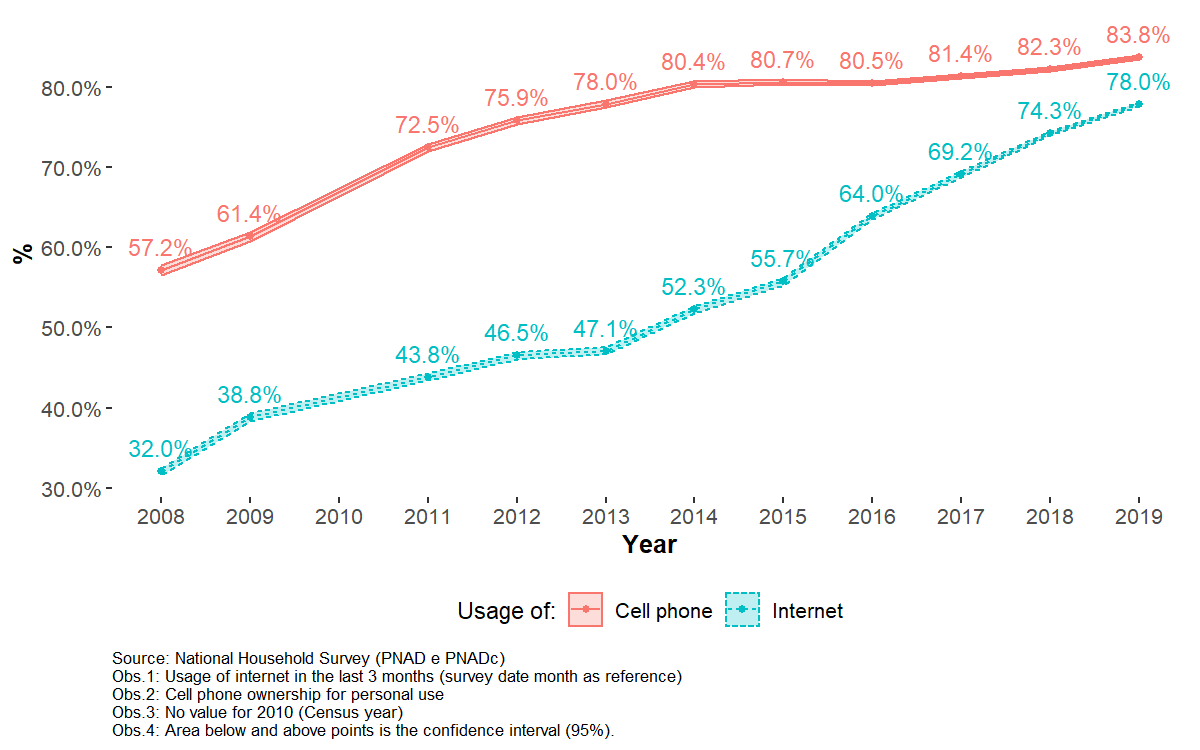
\includegraphics{artigo1_files/figure-latex/internet_usage-1.png}
\caption{Internet and cell phone usage in Brazil, \% of 16+ years-old
population, 2008-2009 and 2011-2018 \label{fig:0}}
\end{figure}

In 2008, around 1/3 of Brazilians (16 years-old or above,
i.e.~population in voting age) declared to have used internet at least
once in the past three months (September as reference), while almost
58\% declared cell phone ownership for personal usage. In order to
increase these figures, the government carried out a national plan in
the begging of 2008. In 2011, these figures rose to 44\% and 73\%,
respectively, indicating an increasing communication market in Brazil.
Even in 2018, there is room remaining for internet and cell phone
expansion in the country (around 25\% and 18\%, respectively).

Hence, this expressive change in communication consumption may have
changed how Brazilians face politics, possibly increasing opportunities
for information acquisition and social interaction about this matter,
or, on the other hand, widening leisure alternatives and lowering
politics information consumption.

\hypertarget{backhaul-program-national-broadband-plan}{%
\subsection{Backhaul Program (National Broadband
Plan)}\label{backhaul-program-national-broadband-plan}}

In April 2008, the presidential Decree 6,424 changed the former National
Plan of Goals for Public Switched Telephone (PST) Network
Universalization, adding broadband infrastructure as mandatory (in
exchange of the PST obligation). The infrastructure mentioned in the
Decree was the Backhaul, a requirement for internet implementation in
the country. Backhauls are necessary in order to connect them to the
Telephone Companies' Backbones. The plan put as target that, at least,
40\% of municipalities should have the necessary infrastructure by the
end of 2008, 80\% by the end of 2009 and 100\% by the end of 2010. Also,
minimal internet velocities were set, increasing with population size
(Table \ref{tab:program_backhauk}).

\begin{table}[!h]

\caption{\label{tab:program_backhauk}Backhaul Plan --  setup}
\centering
\begin{tabu} to \linewidth {>{\raggedright\arraybackslash}p{5.cm}>{\raggedleft}X>{\raggedleft}X>{\raggedleft}X}
\toprule
Population Size & N\# municipalities & \% & Velocity (Mbps)\\
\midrule
Up to 20,000 & 3,077 & 89.5 & 8\\
From 20,001 to 40,000 & 268 & 7.8 & 16\\
From 40,001 to 60,000 & 63 & 1.8 & 32\\
Above 60,001 & 31 & 0.9 & 64\\
Total & 3,439 & 100.0 & \\
\bottomrule
\multicolumn{4}{l}{\rule{0pt}{1em}Source: Anatel}\\
\end{tabu}
\end{table}

According to the National Agency of Telecommunication
(Anatel\footnote{\emph{Agência Nacional de Telecomunicações} in
  Portuguese.}) (Anatel 2010), the majority of municipalities to be
covered by Backhaul program were up to 20,000 inhabitants, which is more
than half of total municipalities of Brazil\footnote{Today, Brazil has
  5,568 municipalities and two districts. By the time when the program
  was created, six municipalities did not exist yet.}. The minimal
required velocity (8 Mbps\footnote{Megabit per second.}) guarantee
improvement in navigation quality, allowing, for example, streaming (of
music and videos).

The program had three types of technology to be deployed: fiber, radio
and satellite. The first is installed by cables of fiber optic, with
less interference and in long distances, being connected directly to the
household (FTTH) or to a concentrating point (FTTC), either with a
higher cost of installation and maintenance. The second one is usually
easier to be installed (by antennas), maintained and reaches broader
areas, like rural locales, but have limitations of interference, due to
physical barriers, and of internet speed, due to distance. Finally, the
third needs a satellite, an antenna in the household and a base antenna
to intermediate communication, a set with high costs of installation and
maintenance, but capable to reach broader areas, like rural, still being
susceptible to weather interference. Considering the costs, radio was
the main technology chosen, for 71\% of the cities, followed by fiber,
for 26\%, and satellite for only 3\%.

Out of 5,570 municipalities, by 2015, only 85 remained uncovered (Table
\ref{tab:desc_back}) and 2,125 (38\%) already had broadband
infrastructure before the program beginning, mainly larger cities. We
notice that the program focused on small cities, with average population
under 15,000.

\begin{table}[!h]

\caption{\label{tab:desc_back}Backhaul deployment by coverage status, 2015}
\centering
\begin{tabu} to \linewidth {>{\raggedright}X>{\raggedleft}X>{\raggedleft}X}
\toprule
Situation & \# Munic & Avg Pop.\\
\midrule
Covered & 3,360 & 14,403\\
Covered before & 2,125 & 67,151\\
Uncovered & 85 & 35,372\\
Total & 5,570 & 34,072\\
\bottomrule
\multicolumn{3}{l}{\rule{0pt}{1em}Source: Anatel and IBGE}\\
\end{tabu}
\end{table}

According to program schedule, 100\% of Brazilians' municipalities
should has backhaul infrastructure in 2010. However, by this year, only
72\% of the goal was achieved. Table \ref{tab:backhaul_implementation}
presents the roll out of the program by year.

\begin{table}[!h]

\caption{\label{tab:backhaul_implementation}Backhaul deployment by year}
\centering
\begin{tabu} to \linewidth {>{\raggedright}X>{\raggedleft}X>{\raggedleft}X>{\raggedleft}X}
\toprule
Backhaul year & \# Munic & Avg. Velocity & Avg Pop.\\
\midrule
2008 & 1,384 & 13 & 16,911\\
2009 & 1,388 & 10 & 13,340\\
2010 & 495 & 9 & 9,026\\
2011 & 27 & 2 & 12,134\\
2012 & 7 & 14 & 25,531\\
2013 & 41 & 4 & 20,238\\
2014 & 17 &  & 38,490\\
2015 & 1 &  & 13,293\\
Total & 3,360 & 11 & 14,403\\
\bottomrule
\multicolumn{4}{l}{\rule{0pt}{1em}Source: Anatel.}\\
\multicolumn{4}{l}{\rule{0pt}{1em}Obs.1: No velocity information for 2014 and 2015.}\\
\multicolumn{4}{l}{\rule{0pt}{1em}Obs.2: Information only for program participants cities.}\\
\end{tabu}
\end{table}

The main point of our identification strategy relies on the velocity
discontinuity, which is further analyzed in Figure \ref{fig:1}
geographically,\footnote{Since Brazil is a continental country
  (8,516,000 km² of area, the fifth in the world) with important
  regional inequalities, regional visualization improve analysis.}.
North and Northeast regions are poorer, while South and Southeast are
richer\footnote{For example, the state of São Paulo was responsible for
  almost 1/3 of Brazilian GDP in 2017. Household income \emph{per
  capita} of the richest state (Federal District) was 3.84 times greater
  than the poorest (Alagoas), according to 2014 National Household
  Survey (IBGE/PNAD). Brazilian Gini index for the same year was 0.517.},
being important to analyze how the programs are deployed in the
territory.

\begin{figure}
\centering
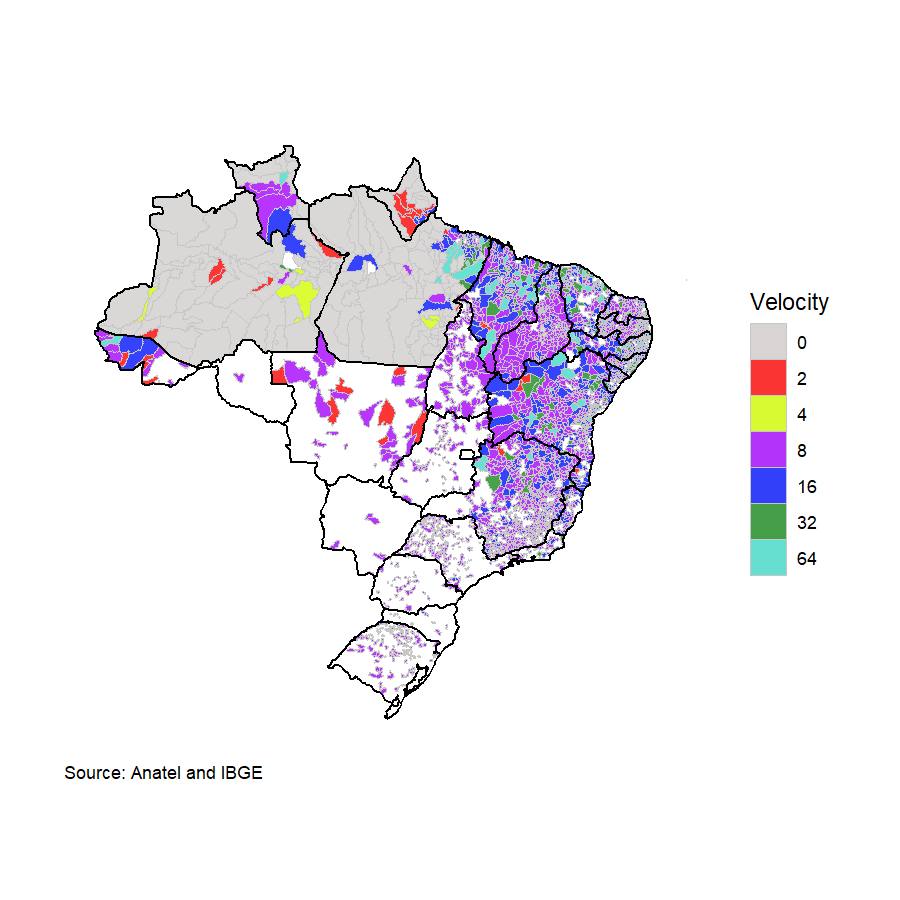
\includegraphics{artigo1_files/figure-latex/unnamed-chunk-1-1.png}
\caption{Internet velocity in backhaul program by municipality
\label{fig:1}}
\end{figure}

Figure \ref{fig:1} shows that a big portion of cities in the south and
center-west were covered before (blank areas), while the northeast had
the largest number of cities in the program. Also, the north region (the
Amazon area) had a lot of cities uncovered by the program (gray areas).
The most common velocity was 8 Mbps, as showed before in Table
\ref{tab:program_backhauk}, corresponding to cities under 20,000
inhabitants.

\hypertarget{methodology}{%
\subsection{Methodology}\label{methodology}}

Following Cattaneo \emph{et al.} (2018), each municipality has a running
variable \(X_i\) (the size of population) with potential outcomes
\(Y_i(0)\) (a lower internet velocity) and \(Y_i(1)\) (higher -- double
-- internet velocity). Municipalities face three possible cutoffs
\(C_i \in C\), with \(C = {c_1, c_2, c_3}\). Ranges of population
determine which type of treatment a municipality will receive: at least
8 Mpbs if \(X_i \leq c_1\), at least 16 Mbps if \(c_1 < X_i \leq c_2\),
at least 32 Mbps if \(c_2 < X_i \leq c_3\) and at least 64 Mbps if
\(X_i > c_3\).

Denote each treatment as \(d_j\), so \(D_i \in \{d_1,d_2,d_3\}\).

The effect for each cutoff, under standard regularity conditions, is
identified by:

\begin{equation}
\tau_j= \mathbb{E}[Y_i(d_j) - Y_i(d_{j-1})|X_i=c_j]= \lim\limits_{x \downarrow c_j}\mathbb{E}[Y_i|X_i=x]-\lim\limits_{x \uparrow c_j}\mathbb{E}[Y_i|X_i=x]
\label{eq:1}
\end{equation}

Each observation may be used to estimate two different, and contiguous,
treatment effects. For example, looking to the first cutoff, 20,000,
municipalities with population above that value are treated (up to the
next cutoff -- 40,000) when estimating \(\tau_j\), but they are controls
when estimating \(\tau_{j+1}\) (and, hence, below the next cutoff --
40,000). An observation can or cannot be used to estimate two effects,
depending on bandwidth selection.

All the three cut-offs are considered (20,000, 40,000 and 60,000), with
optimal bandwidth chosen by minimizing the asymptotic mean squared error
following Calonico \emph{et al.} (2014), Calonico \emph{et al.} (2017)
and Calonico \emph{et al.} (2018).\footnote{Regressions are performed in
  R software, with rdmulti package: Matias D. Cattaneo, Rocio Titiunik
  and Gonzalo Vazquez-Bare (2020). rdmulti: Analysis of RD Designs with
  Multiple Cutoffs or Scores. R package version 0.6.
  \url{https://CRAN.R-project.org/package=rdmulti}}.

Figure \ref{fig:2} shows a clear jump in velocity cutoffs for the entire
period. The jump around cutoffs are clear, where municipalities just
below the population size established in the program face lower internet
velocities.

\begin{figure}
\centering
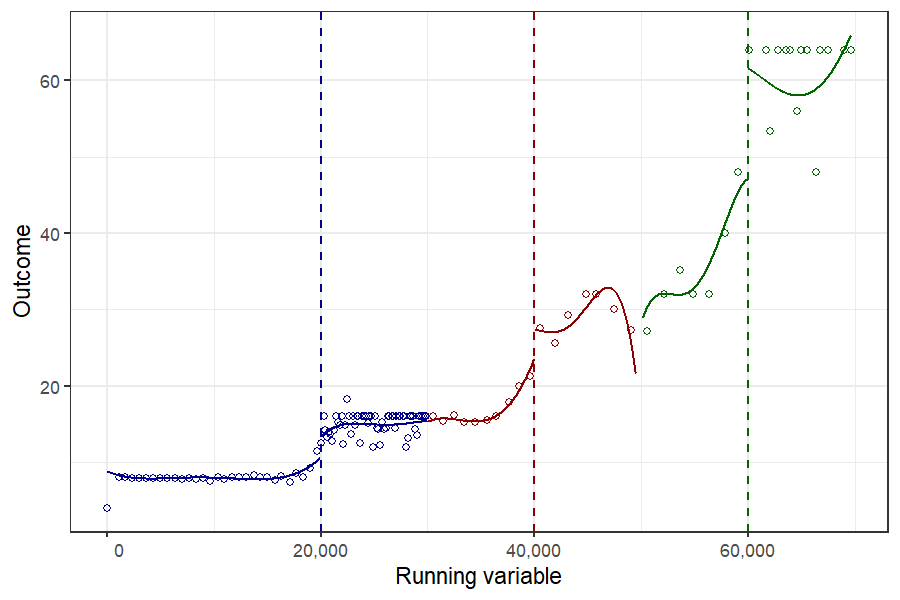
\includegraphics{artigo1_files/figure-latex/discontinuity-1.png}
\caption{Discontinuity in Backhaul program velocity by population
cut-offs: 20,000; 40,000; 60,000 \label{fig:2}}
\end{figure}

The classical McCrary manipulation test of cutoffs (McCrary 2008) looks
if there is a selection into treatment, analyzing the density
distribution of the running variable around the cutoff. An alternative
test was developed by Cattaneo \emph{et al.} (2019) and Cattaneo
\emph{et al.} (2020), where confidence bands are provided, well suited
for RDD designs. Results for this test are presented in Table
\ref{tab:test_tab} Figure \ref{fig:test_plot} for all three cutoffs.

\begin{table}[!h]

\caption{\label{tab:test_tab}Cattaneo, Jansson and Ma manipulation test of cutoffs}
\centering
\resizebox{\linewidth}{!}{
\begin{tabu} to \linewidth {>{\raggedleft}X>{\raggedleft}X>{\raggedleft}X>{\raggedleft}X>{\raggedleft}X>{\raggedleft\arraybackslash}p{3cm}>{\raggedleft}X}
\toprule
Cutoff & Bw & N & Nl & Nr & T (jackknife) & P.value\\
\midrule
20,000 & 4,768 & 3,001 & 305 & 158 & 2.399 & 0.016\\
40,000 & 8,245 & 226 & 120 & 58 & -0.692 & 0.489\\
60,000 & 13,753 & 115 & 47 & 37 & -0.266 & 0.791\\
\bottomrule
\multicolumn{7}{l}{\rule{0pt}{1em}Obs.1: Optimum bandwidht selection following Calonico, Cattaneo and Titiunik (2014).}\\
\multicolumn{7}{l}{\rule{0pt}{1em}Obs.2: Unrestricted density estimation, triangular Kernel and VCE by jackknife.}\\
\multicolumn{7}{l}{\rule{0pt}{1em}Obs.3: Bw=bandwidth; N, Nl and Nr are total n\# of obs., n\# on the left and n\# on the right.}\\
\end{tabu}}
\end{table}

\begin{figure}
\centering
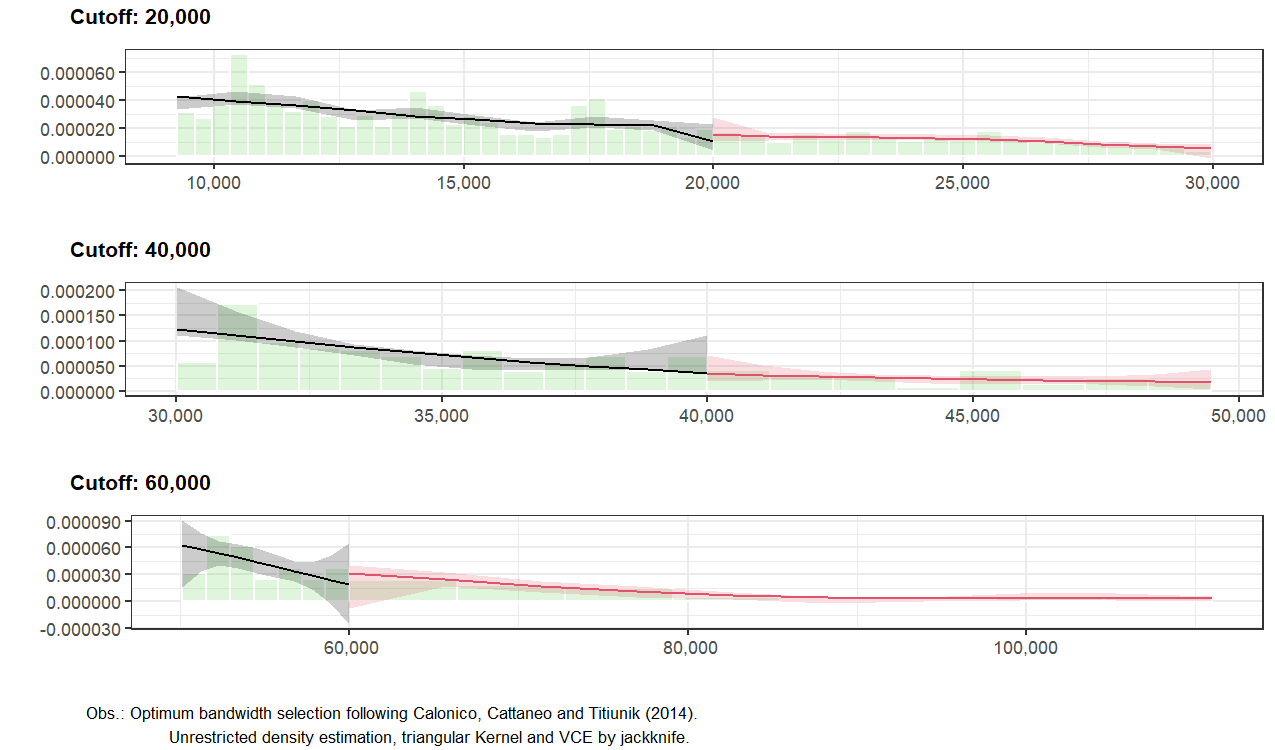
\includegraphics{artigo1_files/figure-latex/test_plot-1.png}
\caption{Density plot - Cattaneo, Jansson and Ma manipulation test of
cutoffs \label{fig:test_plot}}
\end{figure}

The manipulation test, together with Figure \ref{fig:2}, suggests that
our identification strategy is valid, for all three cutoffs, although
the last one in a lower significant level (the cutoff with a lower
number of observations). As we can see on Figure \ref{fig:test_plot},
the visual inspect confirms the test results. Further, the figure shows
that Brazil has an odd population distribution, with unexpected jumps in
some population ranges. Monasterio (2013) shows that these jumps occur
due to a legislation regarding Federal transfers of resources to
municipalities (\emph{Fundo de Participação dos Municípios - FPM}),
based on the population size\footnote{According to the Decree-Law
  1,881/1981, there are 17 ranges of population, with increasing
  possibility of resources distribution for each range. The cuts are:
  10,188; 13,584; 16,980; 23,772; 30,564; 37,356; 44,148; 50,940;
  61,128; 71,316; 81,504; 91,692; 101,880; 115,464; 129,048; 142,632;
  156,216. Available in
  \url{http://www.planalto.gov.br/ccivil_03/Decreto-Lei/1965-1988/Del1881.htm}}.
Despite there are no intersection of running variable and FPM's cutoffs,
we control for the later one, in order to avoid any confounder effect
regarding this situation in results.

\hypertarget{databases}{%
\subsection{Databases}\label{databases}}

Outcomes are election results/information, organized by Superior
Election Court (TSE)\footnote{\emph{Tribunal Superior Eleitoral} in
  Portuguese.}. We will analyze 2008, 2010 and 2012 elections, covering
two municipal and one national suffrage. The main outcomes are: turnout,
percentage of blank or null votes\footnote{In Brazilian election, people
  may put a blank vote, which are not computed for any candidate and is
  not considered for official results, as well null votes. The
  difference consists in the way the registration of these votes are
  made: the blank vote is available as a button in the electronic
  ballot, while the null vote occurs when someone enters an invalid
  candidate number into the ballot and confirms the vote.} and vote
shares, for left wing parties (as mentioned before, and using Power \&
Zucco Jr (2012) party index from Brazilian Legislative
Survey\footnote{Version 7, available in
  \url{https://dataverse.harvard.edu/dataverse/bls;jsessionid=992eedb7e954a17ef718c7078cf5?widget=dataverse\%40harvard\&q=\&types=dataverses\%3Afiles\%3Adatasets\&sort=dateSort\&order=desc\&page=3}},
left wing parties are those up to quantile 0.25 of the index, center
parties are those between 0.25 and 0.75 and right wing are those above),
a small party and young candidates (under 30 years-old). Also, we look
to the number of candidates and the budget campaign of a small party and
young candidates.

Despite the clear discontinuities in the running variable, a set of
covariates were collected, in order to control for any further
confounders that might remain. Lack of information at municipal level is
one of the weakness in Brazilian researches at this territory level.
Census occurs only every ten years\footnote{When not delayed. The 1990
  census was postponed to 1991, as well as 2020 census is postponed to
  2021.}, remaining just few administrative data in the between years,
some of them with low quality (mainly for small cities). Even tough,
considering this is the only source of the main socioeconomic variables,
we use information from the last two censuses (2000 and 2010), organized
by Brazilian Institute of Statistics and Geography (IBGE). Also from
IBGE, we collect total population estimates and GDP. Considering that
direct cash transfers are important in Brazil, we collect data from the
two major programs: \emph{Bolsa Família} (PBF) and \emph{Benefício de
Prestação Continuada} for elders (BPC), booth organized by Ministry of
Citizenship\footnote{PBF is one of the biggest conditional cash transfer
  program in the world. The target are families under the extreme
  poverty and poverty lines (in 2020, families earning up to R\$ 89 by
  person, or U\$ 16, by month are considered extremely poor, while
  families above that amount and up to R\$ 178, or U\$ 32, are
  considered poor), focused one children. As counter part, school
  attendance and vaccination are required. PBF reaches around 14 million
  families in Brazil in 2020. On the other hand, BPC is a program for
  elderly and handicapped. The poor population in this profile (people
  aged 65 or over and all handicapped) are eligible for a minimum wage
  paycheck (R\$ 1.045, or U\$ 185, in 2020).}. In addition, we collect
the mass of wages (formal labor market) from RAIS database, organized by
Ministry of Economy\footnote{In Brazil, every formal company have to
  fill the Annual Relation of Social Information (RAIS), with the
  profile of all workers they had in the calendar year, including wages.}.
We also collected information from National Institute of Meteorology, to
control for rain and temperature in election day, following Fujiwara
\emph{et al.} (2016). Municipalities were joined by the nearest distance
between the center of the city and the closest meteorological station.
Table \ref{tab:variables} summarizes each variable and source.

\begin{table}[!h]

\caption{\label{tab:variables}Variables, description and source, by type}
\centering
\fontsize{9}{11}\selectfont
\begin{tabu} to \linewidth {>{\raggedright\arraybackslash}p{1.5cm}>{\raggedright\arraybackslash}p{3.5cm}>{\raggedright}X>{\raggedright\arraybackslash}p{2.5cm}}
\toprule
Category & Variable & Description & Source\\
\midrule
 & Turnout & Participation percentage of total electorate & TSE\\

 & Vote share & Vote share of parties and/or orientation of parties (left, center or right) & TSE\\

 & Blank and null votes & Percentage of blank and null votes in total & TSE\\

\multirow{-4}{1.5cm}{\raggedright\arraybackslash Outcome} & Donations & Declared donation received for campaign purpose & TSE\\
\cmidrule{1-4}
Running & Population & Estimated population & IBGE\\
\cmidrule{1-4}
 & Black & Percentage of blacks in population & IBGE\\

 & College & Percentage of people with college degree & IBGE\\

 & Married & Percetage of people married & IBGE\\

 & Income & Median household income & IBGE\\

 & Population over 60 years & Percentage of population over 60 years in population & IBGE\\

 & Radio & Percentage of households with radio & IBGE\\

 & Rural & Percentage of population in rural areas & IBGE\\

 & Television & Percentage of households with television & IBGE\\

 & Working age population & Percentage of population in working age & IBGE\\

 & GDP & Gross Domestic Product & IBGE\\

 & BPC & Ratio of BPC payments and GDP & MC and IBGE\\

 & PBF & Ratio of PBF payments and GDP & MC and IBGE\\

 & Formal wage & Ratio of formal wages (sum) and GDP & ME and IBGE\\

 & Temperature & Average temperature a week before and after election day & Inmet\\

 & Rain & Rain preciptation in election day & Inmet\\

 & Fibra-optic & Fibra-optic internet infrasctructure in municipality & Anatel\\

\multirow{-17}{1.5cm}{\raggedright\arraybackslash Controls} & FPM & FPM transfer per capita & Treasury\\
\bottomrule
\multicolumn{4}{l}{\rule{0pt}{1em}Source: TSE, IBGE, Inmet, ME (Ministry of Economy), MC (Ministry of Citizenship) and Anatel.}\\
\end{tabu}
\end{table}

\hypertarget{descriptive-statistics}{%
\subsection{Descriptive statistics}\label{descriptive-statistics}}

Descriptive statistics are separated by population ranges, considering
the cutoffs (under 20,000, between 20,000 and 40,000, between 40,000 and
60,000 and above 60,000). Table \ref{tab:desc.2008} shows the figures
for 2008 year.

\begin{table}[!h]

\caption{\label{tab:desc.2008}Descriptive statistics by population size of municipality, 2008}
\centering
\fontsize{9}{11}\selectfont
\begin{tabu} to \linewidth {>{\raggedright\arraybackslash}p{4cm}>{\raggedright}X>{\raggedright}X>{\raggedright}X>{\raggedright}X}
\toprule
Variable & Under 20k & Above 20k to 40k & Above 40k to 60k & Above 60k\\
\midrule
60\_anos\_2000 & 0.1 & 0.1 & 0.1 & 0.1\\
Avg. Temperature & 24.2 & 25.6 & 26.4 & 27.2\\
Black & 53.4 & 65.5 & 68.1 & 68.6\\
BPC & 0.3 & 0.8 & 0.8 & 0.9\\
College & 0.7 & 0.6 & 0.6 & 0.8\\
Fiber-optic & 23.1 & 34.2 & 33.6 & 47.2\\
Formal Wages & 11.5 & 11.5 & 12.8 & 13.8\\
FPM & 742.9 & 326 & 261.3 & 214.3\\
GDP & 7.8 & 6.9 & 6.3 & 8.2\\
Income & 603.2 & 549.6 & 555.2 & 645.2\\
Married & 30 & 24.1 & 22 & 22.5\\
PBF & 2.5 & 3 & 2.6 & 2\\
pop\_anterior & 8041.5 & 27272.5 & 47975.6 & 97096\\
Radio & 79.3 & 75.4 & 75.6 & 76.1\\
Rain (elect. day) & 3.3 & 1.7 & 1.9 & 2.9\\
Rural & 49.8 & 46.6 & 40.3 & 32.2\\
Television & 69.2 & 66.4 & 68.1 & 73.6\\
Working Pop. & 41.4 & 38.8 & 37.9 & 38.9\\
Observations & 2,733 & 520 & 107 & 72\\
\bottomrule
\multicolumn{5}{l}{\rule{0pt}{1em}Source: IBGE, Inmet, ME, MC and Anatel.}\\
\end{tabu}
\end{table}

We notice that municipalities under 20,000 inhabitants have less
percentage of blacks, BPC transfers and fiber-optic technology
penetration, while more population in working age, in rural areas,
ownership of radio, population over 60 years and married people.

In order to clarify identification validity, Table \ref{tab:t.test}
presents a simple t-test for 20,000 population cutoff with a 3,285
cutoff, the same used before in the manipulation test.

\begin{table}[!h]

\caption{\label{tab:t.test}Covariates means difference t test for 20,000 cutoff, 2008, 2010 and 2012}
\centering
\fontsize{9}{11}\selectfont
\begin{tabu} to \linewidth {>{\raggedright}X>{\raggedright}X>{\raggedright}X>{\raggedright}X}
\toprule
Variable & Diff 2008 & Diff 2010 & Diff 2012\\
\midrule
Median Income & 5.7 & -92.6*** & -38.4\\
Pop. over 60 years & -0.11 & -0.03 & 0.23\\
Rural & 4.59** & 6.84*** & 4.28**\\
Black & -1.51 & 2.44 & 0.29\\
Radio & -1.20 & -1.10 & 0.16\\
Television & -3.48* & -1.91** & -1.11\\
College & 0.03 & -0.26** & -0.16\\
Married & 0.05 & 0.02 & 0.66\\
Working Pop. & -0.73 & -2.22*** & -0.77\\
Rain (elect. day) & -0.2 & 0.1 & 0.0\\
Avg. Temperature & 0.0 & 0.4 & 0.2\\
PBF & 0.24 & 0.67*** & 0.48**\\
BPC & -0.22** & -0.27*** & -0.14\\
GDP & 0.8 & -2.6 & -1.7\\
Formal Wages & -1.73*** & -1.18* & -0.91\\
Fiber-optic & -8.00* & -3.67 & -3.72\\
FPM transfer (pc) & 51.5*** & 53.2*** & 73.4***\\
N. Obs & 380 & 383 & 384\\
\bottomrule
\multicolumn{4}{l}{\rule{0pt}{1em}Source: IBGE, Inmet, ME, MC and Anatel.}\\
\multicolumn{4}{l}{\rule{0pt}{1em}Obs.1: Null hypotheses is no difference.}\\
\multicolumn{4}{l}{\rule{0pt}{1em}Obs.2: * = significant at 10\%; ** = significant at 5\%; *** = significant at 1\%.}\\
\multicolumn{4}{l}{\rule{0pt}{1em}Obs.3: Bandwidth: 3,285}\\
\end{tabu}
\end{table}

Results for 2008 year in Table \ref{tab:t.test} (which, indeed, refers
to 2000 census for socioeconomic variables) show that there were no
significant differences for most of the characteristics between
municipalities just above and just below the cutoff, except for formal
wages (at 1\% of significance), BPC and rural population (at 5\% of
significance), fiber-optic and television (at 10\% of significance).
Some results, however, do not hold in 2010, year with values collected
from 2010 census and, hence, closer to the year of analysis. Some
covariates, like median income, rural areas, working age population BPC
and PBF seems to be different across municipalities, although in a low
absolute difference for the most of then. Results for 2012 is more
similar to those observed in 2000, for the most of variables. Overall,
Table \ref{tab:t.test} results suggests that our identification strategy
should work, if controlled for covariates.

\hypertarget{results}{%
\section{Results}\label{results}}

Considering that there are two rounds for two types of offices, mayor
and president, and some municipalities might not have a second round, we
focus only on the first one, using, hence, the larger sample size as
possible. In tables results, there are always three election years,
where two are local (2008 and 2012) and the other is national (2010). A
summary of first stage of fuzzy RDD regressions are reported in Table
\ref{tab:reg.fs2} in Appendix, all of then supporting the identification
strategy.

We begin our analysis of results looking to the effects of broadband
internet in participation. Results in Table \ref{tab:reg.part} suggest
no relationship between the velocity of this technology and
participation in elections. For all regressions, considering the three
cutoffs and the three years, only one had a slightly significant result
(2010, for 60,000 inhabitants). Since participation in elections is
mandatory in Brazil, and turnout is relatively high (around 80\%), maybe
there is no much room to improve this situation. These results are in
line with Menezes (2015) for Brazil, as well as results reported by
Miner (2015) for Malaysia, but differ from results reported in USA and
European countries (Jaber 2013; Falck \emph{et al.} 2014; Gavazza
\emph{et al.} 2015; Campante \emph{et al.} 2017), where vote is not
mandatory, and, hence, an important institutional difference when
analyzing this result.

\begin{table}[!h]

\caption{\label{tab:reg.part}Fuzzy-RDD regression results for turnout. Election years: 2008, 2010 and 2012}
\centering
\begin{threeparttable}
\begin{tabular}[t]{>{\raggedright\arraybackslash}p{1.9cm}>{\raggedright\arraybackslash}p{1.9cm}>{\raggedleft\arraybackslash}p{1.9cm}>{\raggedleft\arraybackslash}p{1.9cm}>{\raggedleft\arraybackslash}p{1.9cm}>{\raggedleft\arraybackslash}p{1.9cm}>{\raggedleft\arraybackslash}p{1.9cm}}
\toprule
Year & Cutoff & Bw & Obs. & Coef. & SE & P.value\\
\midrule
 & 20,000 & 3,584 & 401 & 0.003 & 0.010 & 0.634\\


 & 40,000 & 11,403 & 265 & 0.003 & 0.004 & 0.229\\


\multirow{-3}{1.9cm}{\raggedright\arraybackslash 2008} & 60,000 & 16,997 & 126 & -0.002 & 0.003 & 0.168\\

\cmidrule{1-7}
 & 20,000 & 4,924 & 554 & -0.001 & 0.006 & 0.493\\


 & 40,000 & 12,191 & 302 & 0.001 & 0.002 & 0.419\\


\multirow{-3}{1.9cm}{\raggedright\arraybackslash 2010} & 60,000 & 23,183 & 200 & 0.002 & 0.001 & 0.071\\

\cmidrule{1-7}
 & 20,000 & 10,735 & 1,335 & 0.002 & 0.003 & 0.507\\


 & 40,000 & 6,617 & 143 & 0.001 & 0.010 & 0.870\\


\multirow{-3}{1.9cm}{\raggedright\arraybackslash 2012} & 60,000 & 11,631 & 95 & 0.001 & 0.003 & 0.649\\
\bottomrule
\end{tabular}
\begin{tablenotes}
\small
\item Obs: Standard Errors (SE) are clustered by regions, with heteroskedasticity-robust nearest neighbor variance estimator (three minimum neighbors). Optimal bandwidth (Bw) selection by Mean Square Error following Calonico, Cattaneo and Titiunik (2014). Triangular kernel with quadratic local-polynomial. Turnout for the first round. Results with controls listed in Table 10
\end{tablenotes}
\end{threeparttable}
\end{table}

Seeing from a different perspective, the new possibility of leisure did
not reduce people participation in elections. In other backgrounds,
where participation in elections are not mandatory, results may be
different (like in Germany and UK, showed by Falck \emph{et al.} (2014)
and Gavazza \emph{et al.} (2015), respectively with negative effects).

The next outcome regards to the percentage of blank or null votes (Table
\ref{tab:r.pct.bn}). Again, there no support in favor of the influence
of broadband internet in this type of votes (a \emph{proxy} for
``absence of engagement with political process'', since these votes can
be seen as a ``whatever vote''). So, results so far suggests that
broadband did not encourage or discourage people to turnout neither
people to place more directed votes in elections (again in accordance to
Menezes (2015) results).

\begin{table}[!h]

\caption{\label{tab:r.pct.bn}RDD-fuzzy regression results for blank or null votes. Election years: 2008, 2010 and 2012. Offices: president and mayors.}
\centering
\begin{threeparttable}
\begin{tabular}[t]{>{\raggedright\arraybackslash}p{1.9cm}>{\raggedright\arraybackslash}p{1.9cm}>{\raggedleft\arraybackslash}p{1.9cm}>{\raggedleft\arraybackslash}p{1.9cm}>{\raggedleft\arraybackslash}p{1.9cm}>{\raggedleft\arraybackslash}p{1.9cm}>{\raggedleft\arraybackslash}p{1.9cm}}
\toprule
Year & Cutoff & Bw & Obs. & Coef. & SE & P.value\\
\midrule
 & 20,000 & 4,250 & 471 & -0.095 & 0.136 & 0.752\\


 & 40,000 & 11,989 & 282 & 0.000 & 0.003 & 0.565\\


\multirow{-3}{1.9cm}{\raggedright\arraybackslash 2008} & 60,000 & 20,209 & 147 & 0.001 & 0.004 & 0.490\\

\cmidrule{1-7}
 & 20,000 & 4,098 & 461 & 0.004 & 0.004 & 0.182\\


 & 40,000 & 9,872 & 251 & 0.002 & 0.004 & 0.320\\


\multirow{-3}{1.9cm}{\raggedright\arraybackslash 2010} & 60,000 & 18,868 & 152 & 0.000 & 0.001 & 0.877\\

\cmidrule{1-7}
 & 20,000 & 3,681 & 413 & 0.023 & 0.027 & 0.196\\


 & 40,000 & 14,408 & 394 & -0.002 & 0.005 & 0.677\\


\multirow{-3}{1.9cm}{\raggedright\arraybackslash 2012} & 60,000 & 13,801 & 107 & 0.034 & 0.170 & 0.822\\
\bottomrule
\end{tabular}
\begin{tablenotes}
\small
\item Obs: Standard Errors (SE) are clustered by regions, with heteroskedasticity-robust nearest neighbor variance estimator (three minimum neighbors). Optimal bandwidth (Bw) selection by Mean Square Error following Calonico, Cattaneo and Titiunik (2014). Triangular kernel with quadratic local-polynomial. Results with controls listed in Table 10
\end{tablenotes}
\end{threeparttable}
\end{table}

In last presidential elections (2018), polarization was dramatic in
Brazil. Left versus Right debate was at the center of the presidential
run, with the last four times presidential winner party (the left wing
Workers Party -- PT) being the main target. Before that, the 2014
elections was one of the closest seen in Brazil, when Mrs.~Rouseff
defeated Mr.~Neves (from central right Brazilian Social Democracy Party
-- PSDB) with only 51.64\% of the valid votes in the second round.
Internet may had an important role in this scenario, since, back in
2010, Mr.~Lula da Silva, the first president of Workers Party, had 80\%
of presidency approval, the highest value ever recorded.\footnote{A news
  about these figures are available in:
  \url{http://g1.globo.com/politica/noticia/2010/12/popularidade-de-lula-bate-recorde-e-chega-87-diz-ibope.html}}

Hence, a closer look at the relationship between broadband velocity and
vote share of left parties since 2008 might shed light into this
turnaround in Brazil. As pointed before, vote shares were classified as
left, center or right based on Power \& Zucco Jr (2012) party index.

Results suggests, once again, that there is no relationship between
broadband internet speed and the vote share received by left wing
parties in elections for president and mayors (Table
\ref{tab:r.pct.vote}). So, unlike results reported by previous studies
(Jaber 2013; Falck \emph{et al.} 2014; Gavazza \emph{et al.} 2015;
Campante \emph{et al.} 2017), there is little evidence of important
effects of internet on vote shares, at least when fixed broadband is
considered.

\begin{table}[!h]

\caption{\label{tab:r.pct.vote}Fuzzy-RDD regression results for left wing parties vote share. Election years: 2008, 2010 and 2012. Offices: president and mayors.}
\centering
\begin{threeparttable}
\begin{tabular}[t]{>{\raggedright\arraybackslash}p{1.9cm}>{\raggedright\arraybackslash}p{1.9cm}>{\raggedleft\arraybackslash}p{1.9cm}>{\raggedleft\arraybackslash}p{1.9cm}>{\raggedleft\arraybackslash}p{1.9cm}>{\raggedleft\arraybackslash}p{1.9cm}>{\raggedleft\arraybackslash}p{1.9cm}}
\toprule
Year & Cutoff & Bw & Obs. & Coef. & SE & P.value\\
\midrule
 & 20,000 & 3,723 & 217 & -0.269 & 2.040 & 0.940\\


 & 40,000 & 12,974 & 195 & -0.009 & 0.034 & 0.919\\


\multirow{-3}{1.9cm}{\raggedright\arraybackslash 2008} & 60,000 & 26,281 & 143 & -0.001 & 0.004 & 0.809\\

\cmidrule{1-7}
 & 20,000 & 4,810 & 542 & -0.003 & 0.011 & 0.820\\


 & 40,000 & 7,651 & 175 & -0.025 & 0.319 & 0.800\\


\multirow{-3}{1.9cm}{\raggedright\arraybackslash 2010} & 60,000 & 21,243 & 183 & 0.003 & 0.003 & 0.243\\

\cmidrule{1-7}
 & 20,000 & 3,693 & 237 & -0.229 & 1.285 & 0.484\\


 & 40,000 & 12,756 & 212 & -0.006 & 0.016 & 0.876\\


\multirow{-3}{1.9cm}{\raggedright\arraybackslash 2012} & 60,000 & 15,286 & 87 & -0.048 & 0.127 & 0.497\\
\bottomrule
\end{tabular}
\begin{tablenotes}
\small
\item Obs: Standard Errors (SE) are clustered by regions, with heteroskedasticity-robust nearest neighbor variance estimator (three minimum neighbors). Optimal bandwidth (Bw) selection by Mean Square Error following Calonico, Cattaneo and Titiunik (2014). Triangular kernel with quadratic local-polynomial. Left wing parties: PSTU, PSOL, PC do B, PT, PSB and PCO. Results with controls listed in Table 10.
\end{tablenotes}
\end{threeparttable}
\end{table}

Despite results suggest no relationship between left wing parties and
votes, some smaller parties, that face narrow campaign budgets, could
use broadband internet to reach more people at lower costs. Table
\ref{tab:r.pct.psol} presents the vote share of PSOL party for local
legislators (\emph{vereador}) and federal deputy (\emph{deputado
federal}), offices with more number of candidates\footnote{Executive
  offices campaigns are more expensive and parties usually support each
  other to improve winning chances, forming blocks (\emph{coligações}).}.
PSOL (\emph{Partido Socialismo e Liberdade}\footnote{Socialism and
  Liberty Party.}) is a relatively recent left wing party, formed in
2004 with dissidents from PT, which makes an interesting case of study.

\begin{table}[!h]

\caption{\label{tab:r.pct.psol}RDD-fuzzy regression results for PSOL vote share. Election years: 2008, 2010 and 2012. Offices: local legislator and federal deputy.}
\centering
\begin{threeparttable}
\begin{tabular}[t]{>{\raggedright\arraybackslash}p{1.9cm}>{\raggedright\arraybackslash}p{1.9cm}>{\raggedleft\arraybackslash}p{1.9cm}>{\raggedleft\arraybackslash}p{1.9cm}>{\raggedleft\arraybackslash}p{1.9cm}>{\raggedleft\arraybackslash}p{1.9cm}>{\raggedleft\arraybackslash}p{1.9cm}}
\toprule
Year & Cutoff & Bw & Obs. & Coef. & SE & P.value\\
\midrule
 & 20,000 & 13,955 & 66 & -0.0016 & 0.0017 & 0.6262\\


 & 40,000 & 27,243 & 84 & 0.0000 & 0.0006 & 0.3531\\


\multirow{-3}{1.9cm}{\raggedright\arraybackslash 2008} & 60,000 & 38,619 & 71 & 0.0009 & 0.0030 & 0.7607\\

\cmidrule{1-7}
 & 20,000 & 6,802 & 772 & -0.0004 & 0.0002 & 0.0119\\


 & 40,000 & 13,581 & 358 & 0.0002 & 0.0002 & 0.0250\\


\multirow{-3}{1.9cm}{\raggedright\arraybackslash 2010} & 60,000 & 20,984 & 179 & -0.0001 & 0.0001 & 0.0789\\

\cmidrule{1-7}
 & 20,000 & 9,708 & 77 & 0.0029 & 0.0187 & 0.8564\\


 & 40,000 & 12,799 & 62 & 0.0003 & 0.0017 & 0.8727\\


\multirow{-3}{1.9cm}{\raggedright\arraybackslash 2012} & 60,000 & 17,647 & 42 & 0.0010 & 0.0038 & 0.5404\\
\bottomrule
\end{tabular}
\begin{tablenotes}
\small
\item Obs: Standard Errors (SE) are clustered by regions, with heteroskedasticity-robust nearest neighbor variance estimator (three minimum neighbors). Optimal bandwidth (Bw) selection by Mean Square Error following Calonico, Cattaneo and Titiunik (2014). Triangular kernel with quadratic local-polynomial. Results with controls listed in Table 10.
\end{tablenotes}
\end{threeparttable}
\end{table}

Results suggests a negative effect, for two out the three cutoffs, in
2010 national elections, but with a limited effect in terms of
percentage of votes. Menezes (2015), reports positive effects for small
and third-placed parties, also for 2010 elections, which is, somewhat
related with results found here, at least in significant results (not in
magnitude or direction).

Another possible effect could be seen in votes for young candidates
(under 30 years), who could take better advantage of broadband internet
due to familiarity to new technologies. Table \ref{tab:r.votos_jovens}
presents the vote share of local legislators (\emph{vereador}) and
federal deputy, who also have more candidates running than for executive
offices.

\begin{table}[!h]

\caption{\label{tab:r.votos_jovens}RDD-fuzzy regression results for young candidates (under 30 years-old). Election years: 2008, 2010 and 2012. Offices: local legislator and federal deputy.}
\centering
\begin{threeparttable}
\begin{tabular}[t]{>{\raggedright\arraybackslash}p{1.9cm}>{\raggedright\arraybackslash}p{1.9cm}>{\raggedleft\arraybackslash}p{1.9cm}>{\raggedleft\arraybackslash}p{1.9cm}>{\raggedleft\arraybackslash}p{1.9cm}>{\raggedleft\arraybackslash}p{1.9cm}>{\raggedleft\arraybackslash}p{1.9cm}}
\toprule
Year & Cutoff & Bw & Obs. & Coef. & SE & P.value\\
\midrule
 & 20,000 & 4,621 & 506 & -0.090 & 0.261 & 0.909\\


 & 40,000 & 13,638 & 333 & 0.004 & 0.006 & 0.180\\


\multirow{-3}{1.9cm}{\raggedright\arraybackslash 2008} & 60,000 & 10,466 & 71 & 0.002 & 0.002 & 0.135\\

\cmidrule{1-7}
 & 20,000 & 3,147 & 368 & 0.009 & 0.014 & 0.288\\


 & 40,000 & 11,604 & 281 & -0.002 & 0.012 & 0.752\\


\multirow{-3}{1.9cm}{\raggedright\arraybackslash 2010} & 60,000 & 7,021 & 55 & 0.000 & 0.001 & 0.795\\

\cmidrule{1-7}
 & 20,000 & 4,319 & 474 & -0.011 & 0.013 & 0.206\\


 & 40,000 & 4,806 & 102 & -0.341 & 25.000 & 0.878\\


\multirow{-3}{1.9cm}{\raggedright\arraybackslash 2012} & 60,000 & 12,816 & 102 & 0.013 & 0.050 & 1.000\\
\bottomrule
\end{tabular}
\begin{tablenotes}
\small
\item Obs: Standard Errors (SE) are clustered by regions, with heteroskedasticity-robust nearest neighbor variance estimator (three minimum neighbors). Optimal bandwidth (Bw) selection by Mean Square Error following Calonico, Cattaneo and Titiunik (2014). Triangular kernel with quadratic local-polynomial. Results with controls listed in Table 10.
\end{tablenotes}
\end{threeparttable}
\end{table}

Results suggests no relationship between broadband internet speed and
vote share for young candidates, in any year or cutoff, meaning that
this technology seems have not helped in electoral performance of
younger.

We now investigate two outcomes not related to ballots directly, but
with candidates participation and budget. Table \ref{tab:r.pct.ncand}
present results for the first, only for 2008 and 2012 years, since in
national elections candidates do not run representing cities or
districts.

\begin{table}[H]

\caption{\label{tab:r.pct.ncand}RDD-fuzzy regression results for number of candidates. Election years: 2008, 2010 and 2012. Offices: local legislator and federal deputy.}
\centering
\begin{threeparttable}
\begin{tabular}[t]{>{\raggedright\arraybackslash}p{1.9cm}>{\raggedright\arraybackslash}p{1.9cm}>{\raggedleft\arraybackslash}p{1.9cm}>{\raggedleft\arraybackslash}p{1.9cm}>{\raggedleft\arraybackslash}p{1.9cm}>{\raggedleft\arraybackslash}p{1.9cm}>{\raggedleft\arraybackslash}p{1.9cm}}
\toprule
Year & Cutoff & Bw & Obs. & Coef. & SE & P.value\\
\midrule
 & 20,000 & 4,309 & 476 & 0.645 & 0.969 & 0.846\\


 & 40,000 & 11,976 & 282 & -0.103 & 0.190 & 0.519\\


\multirow{-3}{1.9cm}{\raggedright\arraybackslash 2008} & 60,000 & 28,290 & 262 & 0.006 & 0.032 & 0.758\\

\cmidrule{1-7}
 & 20,000 & 12,800 & 1,680 & 0.000 & 0.028 & 0.822\\


 & 40,000 & 6,637 & 143 & 0.166 & 0.513 & 0.661\\


\multirow{-3}{1.9cm}{\raggedright\arraybackslash 2012} & 60,000 & 10,808 & 89 & -0.079 & 0.169 & 0.828\\
\bottomrule
\end{tabular}
\begin{tablenotes}
\small
\item Obs: Standard Errors (SE) are clustered by regions, with heteroskedasticity-robust nearest neighbor variance estimator (three minimum neighbors). Optimal bandwidth (Bw) selection by Mean Square Error following Calonico, Cattaneo and Titiunik (2014). Triangular kernel with quadratic local-polynomial. Results with controls listed in Table 10.
\end{tablenotes}
\end{threeparttable}
\end{table}

Like most of the outcomes so far, results suggests no relationship
between broadband internet speed and the number of candidates running
for local offices. The new possibility to reach voters seems not be
sufficient to attract people to run in elections.

Regarding budget campaign, we look two outcomes: the amount used by a
small party (PSOL) and by young candidates (Tables
\ref{tab:r.pct.receita} and \ref{tab:r.receita_jovens}, respectively).

\begin{table}[H]

\caption{\label{tab:r.pct.receita}RDD-fuzzy regression results for PSOL campaign budget Election years: 2008, 2010 and 2012}
\centering
\begin{threeparttable}
\begin{tabular}[t]{>{\raggedright\arraybackslash}p{1.9cm}>{\raggedright\arraybackslash}p{1.9cm}>{\raggedleft\arraybackslash}p{1.9cm}>{\raggedleft\arraybackslash}p{1.9cm}>{\raggedleft\arraybackslash}p{1.9cm}>{\raggedleft\arraybackslash}p{1.9cm}>{\raggedleft\arraybackslash}p{1.9cm}}
\toprule
Year & Cutoff & Bw & Obs. & Coef. & SE & P.value\\
\midrule
 & 20,000 & 19,155 & 58 & 0.053 & 0.266 & 0.725\\


 & 40,000 & 19,261 & 32 & 5.799 & 217.042 & 0.569\\


\multirow{-3}{1.9cm}{\raggedright\arraybackslash 2008} & 60,000 & 28,808 & 26 & 0.037 & 0.199 & 0.941\\

\cmidrule{1-7}
 & 20,000 & 7,267 & 40 & -0.032 & 0.337 & 0.929\\


 & 40,000 & 15,803 & 55 & -0.056 & 0.074 & 0.206\\


\multirow{-3}{1.9cm}{\raggedright\arraybackslash 2012} & 60,000 & 24,205 & 45 & 0.089 & 0.171 & 0.459\\
\bottomrule
\end{tabular}
\begin{tablenotes}
\small
\item Obs: Standard Errors (SE) are clustered by regions, with heteroskedasticity-robust nearest neighbor variance estimator (three minimum neighbors). Optimal bandwidth (Bw) selection by Mean Square Error following Calonico, Cattaneo and Titiunik (2014). Triangular kernel with quadratic local-polynomial. Results with controls listed in Table 10.
\end{tablenotes}
\end{threeparttable}
\end{table}

\begin{table}[H]

\caption{\label{tab:r.receita_jovens}RDD-fuzzy regression results for young candidates (under 30 years-old) budget. Election years: 2008, 2010 and 2012}
\centering
\begin{threeparttable}
\begin{tabular}[t]{>{\raggedright\arraybackslash}p{1.9cm}>{\raggedright\arraybackslash}p{1.9cm}>{\raggedleft\arraybackslash}p{1.9cm}>{\raggedleft\arraybackslash}p{1.9cm}>{\raggedleft\arraybackslash}p{1.9cm}>{\raggedleft\arraybackslash}p{1.9cm}>{\raggedleft\arraybackslash}p{1.9cm}}
\toprule
Year & Cutoff & Bw & Obs. & Coef. & SE & P.value\\
\midrule
 & 20,000 & 4,739 & 524 & -0.157 & 0.603 & 0.838\\


 & 40,000 & 16,976 & 477 & 0.003 & 0.003 & 0.072\\


\multirow{-3}{1.9cm}{\raggedright\arraybackslash 2008} & 60,000 & 11,331 & 73 & 0.001 & 0.002 & 0.694\\

\cmidrule{1-7}
 & 20,000 & 4,892 & 539 & -0.017 & 0.010 & 0.021\\


 & 40,000 & 5,467 & 118 & 0.048 & 0.200 & 0.609\\


\multirow{-3}{1.9cm}{\raggedright\arraybackslash 2012} & 60,000 & 31,060 & 368 & -0.004 & 0.002 & 0.000\\
\bottomrule
\end{tabular}
\begin{tablenotes}
\small
\item Obs: Standard Errors (SE) are clustered by regions, with heteroskedasticity-robust nearest neighbor variance estimator (three minimum neighbors). Optimal bandwidth (Bw) selection by Mean Square Error following Calonico, Cattaneo and Titiunik (2014). Triangular kernel with quadratic local-polynomial. Results with controls listed in Table 10.
\end{tablenotes}
\end{threeparttable}
\end{table}

For the PSOL party, there is no relationship between broadband internet
speed and budget, while for young candidates results are mix: slightly
significant and positive for just one cutoff in 2008 (40,000) and
actually negative in 2012 for the first and last cutoffs. If any
conclusion could be taken is that broadband internet velocity are
related with lower young candidates budgets in 2012 elections. The only
parallel in literature we can make about this outcome is regarding party
donating in US elections, where Jaber (2013) reports a positive impact
for Democratic Party.

\hypertarget{further-investigation}{%
\subsection{Further investigation}\label{further-investigation}}

In the previous section, due to RDD design, each regression was run
considering the multiple cutoff structure. Another way to estimate
results is with parametric regressions, using the distance of the
running variable to the cutoff and adjusting it by a polynomial. We look
to parametric regressions considering two specifications: linear and
quadratic. This choice follows Gelman \& Imbens (2019), to avoid
possible noisy estimates, eventual sensitivity to the degree of the
polynomial and problems with the confidence intervals.

The results are presented in Table \ref{tab:r.par}, with all outcomes
and the three elections years and cutoffs. The lack of relationship
between broadband internet and turnout, blank and null votes, left wing
vote share, number of candidates, PSOL vote share and budget, and young
candidates vote share and budget remains. Significant results are sparse
and, some times, with inverted signs when linear specification is
switched to quadratic.

\begingroup\fontsize{10}{12}\selectfont

\begin{longtable}[t]{>{\raggedright\arraybackslash}p{1.5cm}>{\raggedright\arraybackslash}p{1.5cm}>{\raggedright\arraybackslash}p{1.5cm}>{\raggedleft\arraybackslash}p{1.5cm}>{\raggedleft\arraybackslash}p{1.5cm}>{\raggedleft\arraybackslash}p{1.5cm}>{\raggedleft\arraybackslash}p{1.5cm}>{\raggedright\arraybackslash}p{1.5cm}}
\caption{\label{tab:r.par}Parametric Fuzzy-RDD regression for all outcomes. Election years: 2008, 2010 and 2012}\\
\toprule
Year & Model & Cutoff & Obs. & Coef. & SE & P.value & Outcome\\
\midrule
\endfirsthead
\caption[]{Parametric Fuzzy-RDD regression for all outcomes. Election years: 2008, 2010 and 2012 \textit{(continued)}}\\
\toprule
Year & Model & Cutoff & Obs. & Coef. & SE & P.value & Outcome\\
\midrule
\endhead

\endfoot
\bottomrule
\multicolumn{8}{l}{\rule{0pt}{1em}Obs: Standard Errors (SE) are clustered by regions, with heteroskedasticity-robust variance estimator.}\\
\multicolumn{8}{l}{\rule{0pt}{1em}     Left wing parties: PSTU, PSOL, PC do B, PT, PSB and PCO.}\\
\multicolumn{8}{l}{\rule{0pt}{1em}     Results with controls listed in Table 10.}\\
\endlastfoot
 & Linear & 20,000 & 3,356 & 0.001 & 0.001 & 0.196 & \\
\nopagebreak
 & Quadratic & 20,000 & 3,356 & 0.002 & 0.010 & 0.862 & \\
\nopagebreak
 & Linear & 40,000 & 3,356 & 0.001 & 0.000 & 0.011 & \\
\nopagebreak
 & Quadratic & 40,000 & 3,356 & -0.001 & 0.001 & 0.222 & \\
\nopagebreak
 & Linear & 60,000 & 3,356 & 0.002 & 0.001 & 0.023 & \\
\nopagebreak
\multirow{-6}{1.5cm}{\raggedright\arraybackslash 2008} & Quadratic & 60,000 & 3,356 & -0.001 & 0.001 & 0.061 & \multirow{-6}{1.5cm}{\raggedright\arraybackslash Turnout}\\
\cmidrule{1-8}\pagebreak[0]
 & Linear & 20,000 & 3,427 & 0.001 & 0.001 & 0.089 & \\
\nopagebreak
 & Quadratic & 20,000 & 3,427 & 0.000 & 0.001 & 0.876 & \\
\nopagebreak
 & Linear & 40,000 & 3,427 & 0.000 & 0.000 & 0.010 & \\
\nopagebreak
 & Quadratic & 40,000 & 3,427 & -0.002 & 0.001 & 0.147 & \\
\nopagebreak
 & Linear & 60,000 & 3,427 & 0.002 & 0.000 & 0.000 & \\
\nopagebreak
\multirow{-6}{1.5cm}{\raggedright\arraybackslash 2010} & Quadratic & 60,000 & 3,427 & 0.000 & 0.001 & 0.977 & \multirow{-6}{1.5cm}{\raggedright\arraybackslash Turnout}\\
\cmidrule{1-8}\pagebreak[0]
 & Linear & 20,000 & 3,428 & 0.001 & 0.001 & 0.329 & \\
\nopagebreak
 & Quadratic & 20,000 & 3,428 & 0.000 & 0.001 & 0.579 & \\
\nopagebreak
 & Linear & 40,000 & 3,428 & 0.000 & 0.000 & 0.203 & \\
\nopagebreak
 & Quadratic & 40,000 & 3,428 & -0.002 & 0.001 & 0.132 & \\
\nopagebreak
 & Linear & 60,000 & 3,428 & 0.001 & 0.000 & 0.001 & \\
\nopagebreak
\multirow{-6}{1.5cm}{\raggedright\arraybackslash 2012} & Quadratic & 60,000 & 3,428 & 0.000 & 0.000 & 0.944 & \multirow{-6}{1.5cm}{\raggedright\arraybackslash Turnout}\\
\cmidrule{1-8}\pagebreak[0]
 & Linear & 20,000 & 3,356 & 0.001 & 0.001 & 0.154 & \\
\nopagebreak
 & Quadratic & 20,000 & 3,356 & 0.018 & 0.067 & 0.788 & \\
\nopagebreak
 & Linear & 40,000 & 3,356 & -0.002 & 0.000 & 0.000 & \\
\nopagebreak
 & Quadratic & 40,000 & 3,356 & 0.001 & 0.000 & 0.001 & \\
\nopagebreak
 & Linear & 60,000 & 3,356 & -0.002 & 0.002 & 0.267 & \\
\nopagebreak
\multirow{-6}{1.5cm}{\raggedright\arraybackslash 2008} & Quadratic & 60,000 & 3,356 & 0.001 & 0.002 & 0.590 & \multirow{-6}{1.5cm}{\raggedright\arraybackslash Blank or Null votes}\\
\cmidrule{1-8}\pagebreak[0]
 & Linear & 20,000 & 3,427 & 0.000 & 0.000 & 0.690 & \\
\nopagebreak
 & Quadratic & 20,000 & 3,427 & 0.002 & 0.001 & 0.068 & \\
\nopagebreak
 & Linear & 40,000 & 3,427 & 0.000 & 0.000 & 0.381 & \\
\nopagebreak
 & Quadratic & 40,000 & 3,427 & 0.000 & 0.000 & 0.159 & \\
\nopagebreak
 & Linear & 60,000 & 3,427 & 0.000 & 0.000 & 0.784 & \\
\nopagebreak
\multirow{-6}{1.5cm}{\raggedright\arraybackslash 2010} & Quadratic & 60,000 & 3,427 & 0.001 & 0.000 & 0.009 & \multirow{-6}{1.5cm}{\raggedright\arraybackslash Blank or Null votes}\\
\cmidrule{1-8}\pagebreak[0]
 & Linear & 20,000 & 3,428 & 0.002 & 0.001 & 0.052 & \\
\nopagebreak
 & Quadratic & 20,000 & 3,428 & 0.007 & 0.004 & 0.047 & \\
\nopagebreak
 & Linear & 40,000 & 3,428 & 0.001 & 0.000 & 0.006 & \\
\nopagebreak
 & Quadratic & 40,000 & 3,428 & 0.002 & 0.001 & 0.217 & \\
\nopagebreak
 & Linear & 60,000 & 3,428 & -0.001 & 0.001 & 0.491 & \\
\nopagebreak
\multirow{-6}{1.5cm}{\raggedright\arraybackslash 2012} & Quadratic & 60,000 & 3,428 & -0.002 & 0.001 & 0.182 & \multirow{-6}{1.5cm}{\raggedright\arraybackslash Blank or Null votes}\\
\cmidrule{1-8}\pagebreak[0]
 & Linear & 20,000 & 1,530 & 0.012 & 0.002 & 0.000 & \\
\nopagebreak
 & Quadratic & 20,000 & 1,530 & 0.115 & 0.458 & 0.803 & \\
\nopagebreak
 & Linear & 40,000 & 1,530 & -0.003 & 0.001 & 0.000 & \\
\nopagebreak
 & Quadratic & 40,000 & 1,530 & -0.015 & 0.004 & 0.000 & \\
\nopagebreak
 & Linear & 60,000 & 1,530 & -0.005 & 0.003 & 0.085 & \\
\nopagebreak
\multirow{-6}{1.5cm}{\raggedright\arraybackslash 2008} & Quadratic & 60,000 & 1,530 & -0.012 & 0.008 & 0.145 & \multirow{-6}{1.5cm}{\raggedright\arraybackslash Left wing vote share}\\
\cmidrule{1-8}\pagebreak[0]
 & Linear & 20,000 & 3,427 & 0.001 & 0.001 & 0.575 & \\
\nopagebreak
 & Quadratic & 20,000 & 3,427 & -0.002 & 0.004 & 0.610 & \\
\nopagebreak
 & Linear & 40,000 & 3,427 & 0.001 & 0.001 & 0.586 & \\
\nopagebreak
 & Quadratic & 40,000 & 3,427 & 0.001 & 0.001 & 0.288 & \\
\nopagebreak
 & Linear & 60,000 & 3,427 & 0.000 & 0.001 & 0.960 & \\
\nopagebreak
\multirow{-6}{1.5cm}{\raggedright\arraybackslash 2010} & Quadratic & 60,000 & 3,427 & 0.001 & 0.001 & 0.319 & \multirow{-6}{1.5cm}{\raggedright\arraybackslash Left wing vote share}\\
\cmidrule{1-8}\pagebreak[0]
 & Linear & 20,000 & 1,738 & -0.002 & 0.002 & 0.302 & \\
\nopagebreak
 & Quadratic & 20,000 & 1,738 & -0.011 & 0.012 & 0.371 & \\
\nopagebreak
 & Linear & 40,000 & 1,738 & -0.001 & 0.002 & 0.480 & \\
\nopagebreak
 & Quadratic & 40,000 & 1,738 & -0.004 & 0.002 & 0.058 & \\
\nopagebreak
 & Linear & 60,000 & 1,738 & -0.002 & 0.002 & 0.261 & \\
\nopagebreak
\multirow{-6}{1.5cm}{\raggedright\arraybackslash 2012} & Quadratic & 60,000 & 1,738 & -0.005 & 0.001 & 0.000 & \multirow{-6}{1.5cm}{\raggedright\arraybackslash Left wing vote share}\\
\cmidrule{1-8}\pagebreak[0]
 & Linear & 20,000 & 3,356 & 0.007 & 0.006 & 0.185 & \\
\nopagebreak
 & Quadratic & 20,000 & 3,356 & 0.022 & 0.152 & 0.883 & \\
\nopagebreak
 & Linear & 40,000 & 3,356 & -0.007 & 0.011 & 0.539 & \\
\nopagebreak
 & Quadratic & 40,000 & 3,356 & -0.017 & 0.006 & 0.004 & \\
\nopagebreak
 & Linear & 60,000 & 3,356 & -0.003 & 0.002 & 0.149 & \\
\nopagebreak
\multirow{-6}{1.5cm}{\raggedright\arraybackslash 2008} & Quadratic & 60,000 & 3,356 & 0.010 & 0.012 & 0.401 & \multirow{-6}{1.5cm}{\raggedright\arraybackslash N. cand.}\\
\cmidrule{1-8}\pagebreak[0]
 & Linear & 20,000 & 3,427 & 0.010 & 0.008 & 0.224 & \\
\nopagebreak
 & Quadratic & 20,000 & 3,427 & 0.033 & 0.048 & 0.489 & \\
\nopagebreak
 & Linear & 40,000 & 3,427 & -0.008 & 0.010 & 0.466 & \\
\nopagebreak
 & Quadratic & 40,000 & 3,427 & -0.006 & 0.014 & 0.658 & \\
\nopagebreak
 & Linear & 60,000 & 3,427 & -0.018 & 0.010 & 0.070 & \\
\nopagebreak
\multirow{-6}{1.5cm}{\raggedright\arraybackslash 2012} & Quadratic & 60,000 & 3,427 & -0.014 & 0.009 & 0.101 & \multirow{-6}{1.5cm}{\raggedright\arraybackslash N. cand.}\\
\cmidrule{1-8}\pagebreak[0]
 & Linear & 20,000 & 128 & 0.000 & 0.001 & 0.370 & \\
\nopagebreak
 & Quadratic & 20,000 & 128 & 0.002 & 0.001 & 0.225 & \\
\nopagebreak
 & Linear & 40,000 & 128 & 0.001 & 0.001 & 0.089 & \\
\nopagebreak
 & Quadratic & 40,000 & 128 & 0.000 & 0.000 & 0.038 & \\
\nopagebreak
 & Linear & 60,000 & 128 & 0.002 & 0.005 & 0.652 & \\
\nopagebreak
\multirow{-6}{1.5cm}{\raggedright\arraybackslash 2008} & Quadratic & 60,000 & 128 & 0.000 & 0.004 & 0.915 & \multirow{-6}{1.5cm}{\raggedright\arraybackslash PSOL vote share}\\
\cmidrule{1-8}\pagebreak[0]
 & Linear & 20,000 & 2,815 & 0.000 & 0.000 & 0.266 & \\
\nopagebreak
 & Quadratic & 20,000 & 2,815 & 0.000 & 0.000 & 0.002 & \\
\nopagebreak
 & Linear & 40,000 & 2,815 & 0.000 & 0.000 & 0.719 & \\
\nopagebreak
 & Quadratic & 40,000 & 2,815 & 0.000 & 0.000 & 0.003 & \\
\nopagebreak
 & Linear & 60,000 & 2,815 & 0.000 & 0.000 & 0.765 & \\
\nopagebreak
\multirow{-6}{1.5cm}{\raggedright\arraybackslash 2010} & Quadratic & 60,000 & 2,815 & 0.000 & 0.000 & 0.629 & \multirow{-6}{1.5cm}{\raggedright\arraybackslash PSOL vote share}\\
\cmidrule{1-8}\pagebreak[0]
 & Linear & 20,000 & 211 & -0.001 & 0.001 & 0.363 & \\
\nopagebreak
 & Quadratic & 20,000 & 211 & -0.003 & 0.009 & 0.708 & \\
\nopagebreak
 & Linear & 40,000 & 211 & 0.000 & 0.000 & 0.018 & \\
\nopagebreak
 & Quadratic & 40,000 & 211 & 0.000 & 0.000 & 0.770 & \\
\nopagebreak
 & Linear & 60,000 & 211 & 0.000 & 0.000 & 0.024 & \\
\nopagebreak
\multirow{-6}{1.5cm}{\raggedright\arraybackslash 2012} & Quadratic & 60,000 & 211 & 0.000 & 0.000 & 0.410 & \multirow{-6}{1.5cm}{\raggedright\arraybackslash PSOL vote share}\\
\cmidrule{1-8}\pagebreak[0]
 & Linear & 20,000 & 89 & 0.245 & 0.350 & 0.484 & \\
\nopagebreak
 & Quadratic & 20,000 & 89 & -0.430 & 1.099 & 0.696 & \\
\nopagebreak
 & Linear & 40,000 & 89 & -0.007 & 0.036 & 0.855 & \\
\nopagebreak
 & Quadratic & 40,000 & 89 & -0.049 & 0.019 & 0.010 & \\
\nopagebreak
 & Linear & 60,000 & 89 & 0.082 & 0.109 & 0.450 & \\
\nopagebreak
\multirow{-6}{1.5cm}{\raggedright\arraybackslash 2008} & Quadratic & 60,000 & 89 & 0.162 & 0.109 & 0.137 & \multirow{-6}{1.5cm}{\raggedright\arraybackslash PSOL budget}\\
\cmidrule{1-8}\pagebreak[0]
 & Linear & 20,000 & 149 & -0.006 & 0.021 & 0.776 & \\
\nopagebreak
 & Quadratic & 20,000 & 149 & -0.016 & 0.117 & 0.894 & \\
\nopagebreak
 & Linear & 40,000 & 149 & -0.046 & 0.007 & 0.000 & \\
\nopagebreak
 & Quadratic & 40,000 & 149 & -0.141 & 0.033 & 0.000 & \\
\nopagebreak
 & Linear & 60,000 & 149 & 0.029 & 0.016 & 0.079 & \\
\nopagebreak
\multirow{-6}{1.5cm}{\raggedright\arraybackslash 2012} & Quadratic & 60,000 & 149 & 0.044 & 0.039 & 0.265 & \multirow{-6}{1.5cm}{\raggedright\arraybackslash PSOL budget}\\
\cmidrule{1-8}\pagebreak[0]
 & Linear & 20,000 & 3,237 & 0.002 & 0.002 & 0.258 & \\
\nopagebreak
 & Quadratic & 20,000 & 3,237 & 0.014 & 0.038 & 0.720 & \\
\nopagebreak
 & Linear & 40,000 & 3,237 & 0.001 & 0.001 & 0.104 & \\
\nopagebreak
 & Quadratic & 40,000 & 3,237 & 0.001 & 0.002 & 0.489 & \\
\nopagebreak
 & Linear & 60,000 & 3,237 & -0.001 & 0.001 & 0.525 & \\
\nopagebreak
\multirow{-6}{1.5cm}{\raggedright\arraybackslash 2008} & Quadratic & 60,000 & 3,237 & -0.002 & 0.001 & 0.006 & \multirow{-6}{1.5cm}{\raggedright\arraybackslash Young votes}\\
\cmidrule{1-8}\pagebreak[0]
 & Linear & 20,000 & 3,413 & 0.001 & 0.001 & 0.139 & \\
\nopagebreak
 & Quadratic & 20,000 & 3,413 & 0.001 & 0.004 & 0.800 & \\
\nopagebreak
 & Linear & 40,000 & 3,413 & 0.000 & 0.000 & 0.419 & \\
\nopagebreak
 & Quadratic & 40,000 & 3,413 & -0.001 & 0.000 & 0.012 & \\
\nopagebreak
 & Linear & 60,000 & 3,413 & -0.001 & 0.000 & 0.004 & \\
\nopagebreak
\multirow{-6}{1.5cm}{\raggedright\arraybackslash 2010} & Quadratic & 60,000 & 3,413 & -0.002 & 0.000 & 0.000 & \multirow{-6}{1.5cm}{\raggedright\arraybackslash Young votes}\\
\cmidrule{1-8}\pagebreak[0]
 & Linear & 20,000 & 3,369 & -0.001 & 0.001 & 0.098 & \\
\nopagebreak
 & Quadratic & 20,000 & 3,369 & -0.008 & 0.006 & 0.172 & \\
\nopagebreak
 & Linear & 40,000 & 3,369 & -0.001 & 0.001 & 0.390 & \\
\nopagebreak
 & Quadratic & 40,000 & 3,369 & -0.001 & 0.002 & 0.699 & \\
\nopagebreak
 & Linear & 60,000 & 3,369 & 0.000 & 0.000 & 0.090 & \\
\nopagebreak
\multirow{-6}{1.5cm}{\raggedright\arraybackslash 2012} & Quadratic & 60,000 & 3,369 & -0.001 & 0.001 & 0.322 & \multirow{-6}{1.5cm}{\raggedright\arraybackslash Young votes}\\
\cmidrule{1-8}\pagebreak[0]
 & Linear & 20,000 & 3,237 & 0.001 & 0.003 & 0.828 & \\
\nopagebreak
 & Quadratic & 20,000 & 3,237 & 0.015 & 0.060 & 0.800 & \\
\nopagebreak
 & Linear & 40,000 & 3,237 & 0.001 & 0.001 & 0.100 & \\
\nopagebreak
 & Quadratic & 40,000 & 3,237 & 0.002 & 0.002 & 0.305 & \\
\nopagebreak
 & Linear & 60,000 & 3,237 & 0.000 & 0.001 & 0.961 & \\
\nopagebreak
\multirow{-6}{1.5cm}{\raggedright\arraybackslash 2008} & Quadratic & 60,000 & 3,237 & -0.001 & 0.002 & 0.641 & \multirow{-6}{1.5cm}{\raggedright\arraybackslash Young budget}\\
\cmidrule{1-8}\pagebreak[0]
 & Linear & 20,000 & 3,369 & -0.002 & 0.000 & 0.000 & \\
\nopagebreak
 & Quadratic & 20,000 & 3,369 & -0.011 & 0.009 & 0.230 & \\
\nopagebreak
 & Linear & 40,000 & 3,369 & 0.000 & 0.000 & 0.441 & \\
\nopagebreak
 & Quadratic & 40,000 & 3,369 & 0.000 & 0.001 & 0.866 & \\
\nopagebreak
 & Linear & 60,000 & 3,369 & -0.001 & 0.000 & 0.167 & \\
\nopagebreak
\multirow{-6}{1.5cm}{\raggedright\arraybackslash 2012} & Quadratic & 60,000 & 3,369 & -0.002 & 0.001 & 0.026 & \multirow{-6}{1.5cm}{\raggedright\arraybackslash Young budget}\\*
\end{longtable}
\endgroup{}

The only result we could point out as relatively consistent is the
negative relationship between the internet velocity and left wing vote
share, for local elections (2008 and 2010) and for the 40,000 cutoff.
But, being too specific, it is hard to support this results as
consistent, specially taking into considerations the results in previous
section.

A possible limitation of RDD models is the bandwidth choice, which could
influence results. It is possible that a narrower or wider bandwidth
give different results, since fewer or more observations will be part of
regressions (a trade off between ``randomness'' and ``precision'').
Considering this possibility, Table \ref{tab:r.sig} presents only
significant results using also half or double bandwidths of those used
in the previous section.

\begingroup\fontsize{10}{12}\selectfont

\begin{longtable}[t]{>{\raggedright\arraybackslash}p{1.4cm}>{\raggedright\arraybackslash}p{1.4cm}>{\raggedright\arraybackslash}p{1.8cm}>{\raggedleft\arraybackslash}p{1.4cm}>{\raggedleft\arraybackslash}p{1.4cm}>{\raggedleft\arraybackslash}p{1.4cm}>{\raggedleft\arraybackslash}p{1.4cm}>{\raggedright\arraybackslash}p{3.5cm}}
\caption{\label{tab:r.sig}Significant Fuzzy-RDD regression with half or double bandwidths for all outcomes. Election years: 2008, 2010 and 2012}\\
\toprule
Year & Cutoff & Model & Obs. & Coef. & SE & P.value & Outcome\\
\midrule
\endfirsthead
\caption[]{Significant Fuzzy-RDD regression with half or double bandwidths for all outcomes. Election years: 2008, 2010 and 2012 \textit{(continued)}}\\
\toprule
Year & Cutoff & Model & Obs. & Coef. & SE & P.value & Outcome\\
\midrule
\endhead

\endfoot
\bottomrule
\multicolumn{8}{l}{\rule{0pt}{1em}Obs: Standard Errors (SE) are clustered by regions, with heteroskedasticity-robust variance estimator.}\\
\multicolumn{8}{l}{\rule{0pt}{1em}     Left wing parties: PSTU, PSOL, PC do B, PT, PSB and PCO.}\\
\multicolumn{8}{l}{\rule{0pt}{1em}     Results with controls listed in Table 10.}\\
\endlastfoot
2008 & 60,000 & Double-Bw & 423 & 0.000 & 0.001 & 0.010 & Turnout\\
\cmidrule{1-8}\pagebreak[0]
 & 60,000 & Half-Bw & 88 & 0.002 & 0.004 & 0.099 & \\
\nopagebreak
\multirow{-2}{1.4cm}{\raggedright\arraybackslash 2010} & 60,000 & Double-Bw & 1,214 & 0.001 & 0.001 & 0.000 & \multirow{-2}{3.5cm}{\raggedright\arraybackslash Turnout}\\
\cmidrule{1-8}\pagebreak[0]
2008 & 20,000 & Double-Bw & 549 & 0.013 & 0.010 & 0.001 & Blank or Null votes\\
\cmidrule{1-8}\pagebreak[0]
2010 & 20,000 & Half-Bw & 242 & 0.006 & 0.008 & 0.081 & Blank or Null votes\\
\cmidrule{1-8}\pagebreak[0]
 & 20,000 & Double-Bw & 519 & 0.002 & 0.002 & 0.000 & \\
\nopagebreak
 & 40,000 & Half-Bw & 103 & -0.013 & 0.037 & 0.087 & \\
\nopagebreak
\multirow{-3}{1.4cm}{\raggedright\arraybackslash 2012} & 60,000 & Double-Bw & 195 & -0.006 & 0.005 & 0.002 & \multirow{-3}{3.5cm}{\raggedright\arraybackslash Blank or Null votes}\\
\cmidrule{1-8}\pagebreak[0]
2008 & 40,000 & Double-Bw & 1,092 & 0.023 & 0.043 & 0.058 & Left wing vote share\\
\cmidrule{1-8}\pagebreak[0]
 & 20,000 & Half-Bw & 191 & 0.351 & 0.804 & 0.029 & \\
\nopagebreak
\multirow{-2}{1.4cm}{\raggedright\arraybackslash 2012} & 60,000 & Half-Bw & 65 & -0.022 & 0.021 & 0.051 & \multirow{-2}{3.5cm}{\raggedright\arraybackslash Left wing vote share}\\
\cmidrule{1-8}\pagebreak[0]
2008 & 20,000 & Double-Bw & 1,031 & -0.103 & 0.097 & 0.000 & N. cand.\\
\cmidrule{1-8}\pagebreak[0]
 & 20,000 & Double-Bw & 1,687 & 0.000 & 0.000 & 0.000 & \\
\nopagebreak
\multirow{-2}{1.4cm}{\raggedright\arraybackslash 2010} & 60,000 & Double-Bw & 848 & 0.000 & 0.000 & 0.008 & \multirow{-2}{3.5cm}{\raggedright\arraybackslash PSOL vote share}\\
\cmidrule{1-8}\pagebreak[0]
 & 20,000 & Double-Bw & 1,097 & 0.006 & 0.014 & 0.099 & \\
\nopagebreak
\multirow{-2}{1.4cm}{\raggedright\arraybackslash 2008} & 60,000 & Double-Bw & 153 & 0.000 & 0.002 & 0.004 & \multirow{-2}{3.5cm}{\raggedright\arraybackslash Young votes}\\
\cmidrule{1-8}\pagebreak[0]
 & 20,000 & Half-Bw & 226 & 0.004 & 0.056 & 0.078 & \\
\nopagebreak
 & 20,000 & Double-Bw & 1,031 & -0.006 & 0.004 & 0.028 & \\
\nopagebreak
\multirow{-3}{1.4cm}{\raggedright\arraybackslash 2012} & 60,000 & Double-Bw & 248 & -0.004 & 0.005 & 0.029 & \multirow{-3}{3.5cm}{\raggedright\arraybackslash Young votes}\\
\cmidrule{1-8}\pagebreak[0]
 & 20,000 & Double-Bw & 1,127 & 0.010 & 0.020 & 0.070 & \\
\nopagebreak
\multirow{-2}{1.4cm}{\raggedright\arraybackslash 2008} & 40,000 & Double-Bw & 2,098 & 0.032 & 0.136 & 0.075 & \multirow{-2}{3.5cm}{\raggedright\arraybackslash Young budget}\\
\cmidrule{1-8}\pagebreak[0]
 & 20,000 & Double-Bw & 1,242 & -0.008 & 0.003 & 0.000 & \\
\nopagebreak
\multirow{-2}{1.4cm}{\raggedright\arraybackslash 2012} & 60,000 & Double-Bw & 3,359 & -0.001 & 0.000 & 0.000 & \multirow{-2}{3.5cm}{\raggedright\arraybackslash Young budget}\\*
\end{longtable}
\endgroup{}

Once again significant results are sparse, for some years, outcome,
cutoffs and bandwidths, putting in check any solid relationship between
broadband internet speed and election outcomes.

\hypertarget{pooled-regressions}{%
\subsubsection{Pooled regressions}\label{pooled-regressions}}

The cumulative RDD regression design, although considers all the
heterogeneity that multiple cutoffs offers, reduces the sample size,
specially in the 40,000 and 60,000 cutoffs. We now look for pooled
regressions, in order to verify if combined samples (and, hence, more
observations) support results presented in the previous sections. All
cutoffs are considered, and samples are divided by the mean value
between the cutoffs (population up to 30,000 for the first, between
30,001 and 50,000 for the second and 50,001 and above for the third).
Results for all outcomes are presented in Table \ref{tab:r.pooled}.

\begin{table}[!h]

\caption{\label{tab:r.pooled}RDD-fuzzy pooled regressions for all outcomes. Election years: 2008, 2010 and 2012}
\centering
\begin{threeparttable}
\begin{tabular}[t]{>{\raggedright\arraybackslash}p{1.9cm}>{\raggedleft\arraybackslash}p{1.9cm}>{\raggedleft\arraybackslash}p{1.9cm}>{\raggedleft\arraybackslash}p{1.9cm}>{\raggedleft\arraybackslash}p{1.9cm}>{\raggedleft\arraybackslash}p{1.9cm}>{\raggedright\arraybackslash}p{1.9cm}}
\toprule
Year & Bw & Obs. & Coef. & SE & P.value & Outcome\\
\midrule
2008 & 3,435 & 476 & 0.001 & 0.008 & 0.786 & \\

2010 & 3,559 & 510 & -0.009 & 0.007 & 0.068 & \\

2012 & 4,379 & 605 & 0.013 & 0.010 & 0.121 & \multirow{-3}{1.9cm}{\raggedright\arraybackslash Turnout}\\
\cmidrule{1-7}
2008 & 3,727 & 506 & 0.051 & 0.010 & 0.000 & \\

2010 & 4,770 & 676 & 0.008 & 0.005 & 0.063 & \\

2012 & 3,513 & 499 & 0.008 & 0.019 & 0.531 & \multirow{-3}{1.9cm}{\raggedright\arraybackslash Blank or Null votes}\\
\cmidrule{1-7}
2008 & 3,672 & 275 & 0.102 & 0.033 & 0.001 & \\

2010 & 4,784 & 676 & -0.002 & 0.021 & 0.869 & \\

2012 & 2,246 & 188 & -0.096 & 0.027 & 0.000 & \multirow{-3}{1.9cm}{\raggedright\arraybackslash Left wing vote share}\\
\cmidrule{1-7}
2008 & 2,281 & 315 & -0.636 & 0.117 & 0.000 & \\

2012 & 3,614 & 509 & 0.200 & 0.127 & 0.053 & \multirow{-2}{1.9cm}{\raggedright\arraybackslash N. cand.}\\
\cmidrule{1-7}
2008 & 3,684 & 28 & -0.003 & 0.011 & 0.801 & \\

2010 & 7,764 & 1,131 & -0.001 & 0.001 & 0.113 & \\

2012 & 3,915 & 65 & -0.002 & 0.005 & 0.257 & \multirow{-3}{1.9cm}{\raggedright\arraybackslash PSOL vote share}\\
\cmidrule{1-7}
2008 & 4,311 & 27 & 1.496 & 0.522 & 0.003 & \\

2012 & 3,138 & 40 & 2.840 & 0.519 & 0.000 & \multirow{-2}{1.9cm}{\raggedright\arraybackslash PSOL budget}\\
\cmidrule{1-7}
2008 & 3,476 & 477 & 0.039 & 0.029 & 0.102 & \\

2010 & 4,650 & 655 & -0.009 & 0.009 & 0.318 & \\

2012 & 7,498 & 1,116 & -0.016 & 0.027 & 0.600 & \multirow{-3}{1.9cm}{\raggedright\arraybackslash Young votes}\\
\cmidrule{1-7}
2008 & 3,894 & 517 & 0.053 & 0.029 & 0.031 & \\

2012 & 5,954 & 867 & -0.022 & 0.012 & 0.085 & \multirow{-2}{1.9cm}{\raggedright\arraybackslash Young budget}\\
\bottomrule
\end{tabular}
\begin{tablenotes}
\small
\item Obs: Standard Errors (SE) are clustered by regions, with heteroskedasticity-robust nearest neighbor variance estimator (three minimum neighbors). Optimal bandwidth (Bw) selection by Mean Square Error following Calonico, Cattaneo and Titiunik (2014). Triangular kernel with quadratic local-polynomial. Results with controls listed in Table 10.
\end{tablenotes}
\end{threeparttable}
\end{table}

Results suggest a negative effect for turnout in 2010 and positive
effects for blank or null votes in 2008 and 2010. Regarding left wing
vote share, a positive effect in 2008 is reverted to negative in 2012.
PSOL vote share is no longer significant, while its budget is. In 2008,
we see a negative effect to number of candidates, reverting to positive
in 2012. Finally, for younger candidates, we observe no effects on
votes, but a significant effects on budget: positive in 2008 reverted to
negative in 2012.

Putting all these results together (the cumulative RDD, the parametric
RDD and the pooled RDD), it is hard to conclude that the Backhaul
program, and, hence, broadband internet velocity, made a significant
difference in 2008, 2010 and 2012 elections in terms of turnout,
percentage of blank or null votes, left wing vote share, PSOL vote
share, young candidates vote share and PSOL and young candidates budget.
Although only the first round and four offices were analyzed, it is not
likely to see a different results in other scenarios (second rounds and
other offices). The lack of consistency across specification, years and
cutoffs put in check the significant results observed in some
regressions.

\hypertarget{discussion-and-conclusions}{%
\section{Discussion and conclusions}\label{discussion-and-conclusions}}

Relationship between broadband velocity and elections outcome did not
seems be relevant in Brazil, at least when fixed broadband are
considered, neither for local or national elections between 2008 and
2012. Despite our robust identification strategy, we did not find strong
relationship between broadband velocity, measured by the jumps of
internet speed in the Backhaul program roll out, and election outcomes.
These results are in line with some finds reported by Menezes (2015)
(turnout and blank and null votes), but differs from others (vote
shares).

Our results are also different from those reported in some part of the
literature, mostly concentrated in European countries and USA (Jaber
2013; Falck \emph{et al.} 2014; Gavazza \emph{et al.} 2015; Campante
\emph{et al.} 2017), which could indicate that the background may be
important in this kind of analysis. First of all, vote is mandatory in
Brazil, which is not necessarily true in other countries. Second, the
political system in Brazil is presidentialist, in a federation republic,
which means that people may behavior differently than in a
parliamentarian system. Third, national congress deputies and local
assemblies are elected by proportional vote, while senators are elected
by majority vote, situation that may differ across countries. A fourth
source of variation in political background regards to the difference
between unitary and federal systems, that sets different rules to be
played in the ``political game''.

Aside the political background, the internet usage is not fully
controlled in our analysis. Installing the internet infrastructure in a
municipality does not mean that all population will have access to the
technology. Figure \ref{fig:0} shows that less than a third of Brazilian
population had access to the internet in 2008, rising to 46.5\% in 2012.
Despite the lower costs internet provide in electoral campaign, less
than half of population could be reached until 2012, even a less portion
in poorer cities. So, it might be the case that internet velocity had a
limited room to change reality and the sparse significant results found
is not sufficient to trace a pattern yet.

Also, it was not possible to addressed the qualification of internet
usage in our analysis. First of all, social networks have grown in
Brazil after 2010. WhatsApp, one of the most popular social network in
Brazil today, was created only in 2009, the very same year internet
campaign was regulated. Is it possible that, today, mobile broadband and
social medias usage in smartphones are more important for communication
and mobilization than older social medias and connection made at home,
through desktop or laptop computers and by fixed land lines.
Unfortunately, the roll out of 3G and 4G technology implementation, at
municipality level, is unavailable. There is only data at Direct
Dialling codes (DDDs)\footnote{The DDD codes are numbers that divides
  Brazil in 67 areas.} areas, which makes impossible to determine when
the technology begun to operate in every city\footnote{We contacted the
  Regulation Agency of Telecommunication -- Anatel -- requesting mobile
  internet implementation at municipality level. Unfortunately, there is
  no such data available.}.

Nonetheless, our paper contributes to bring into discussion that
internet and political outcomes should be viewed in a wider perspective,
meaning that some relationship may be circumstantial to idiosyncrasies
of the countries or the technology. Also, further investigation, like
the role of the new social medias and mobile broadband, are necessary to
shed light in this discussion, even because internet and social medias
are still evolving.

\hypertarget{references}{%
\section*{References}\label{references}}
\addcontentsline{toc}{section}{References}

\hypertarget{refs}{}
\begin{CSLReferences}{1}{0}
\leavevmode\hypertarget{ref-aldrich_rational_1993}{}%
Aldrich, J.H. (1993). Rational choice and turnout. \emph{American
journal of political science}, 246--278.

\leavevmode\hypertarget{ref-ali_why_2013}{}%
Ali, S.N. \& Lin, C. (2013). Why people vote: {Ethical} motives and
social incentives. \emph{American economic Journal: microeconomics},
\textbf{5}, 73--98.

\leavevmode\hypertarget{ref-allcott_social_2017}{}%
Allcott, H. \& Gentzkow, M. (2017). Social media and fake news in the
2016 election. \emph{Journal of economic perspectives}, \textbf{31},
211--36.

\leavevmode\hypertarget{ref-anatel_relatorio_2010}{}%
Anatel. (2010). {RELATÓRIO} {DE} {ACOMPANHAMENTO} {DAS} {METAS} {DE}
{IMPLEMENTAÇÃO} {DA} {INFRAESTRUTURA} {DE} {REDE} {DE} {SUPORTE} {DO}
{STFC} {PARA} {CONEXÃO} {EM} {BANDA} {LARGA} ({BACKHAUL}).

\leavevmode\hypertarget{ref-banerjee_informed_2011}{}%
Banerjee, A., Kumar, S., Pande, R. \& Su, F. (2011). Do informed voters
make better choices? {Experimental} evidence from urban {India}.
\emph{Unpublished manuscript}. Retrieved June 4, 2017, from
\url{https://pdfs.semanticscholar.org/fc45/db4976c51fd67177757ca895896c3a01039e.pdf}

\leavevmode\hypertarget{ref-besley_handcuffs_2006}{}%
Besley, T. \& Prat, A. (2006). Handcuffs for the grabbing hand? {Media}
capture and government accountability. \emph{American economic review},
\textbf{96}, 720--736.

\leavevmode\hypertarget{ref-bimber_information_2003}{}%
Bimber, B. (2003). \emph{Information and {American} democracy:
{Technology} in the evolution of political power}. Cambridge University
Press.

\leavevmode\hypertarget{ref-bimber_internet_1998}{}%
Bimber, B. (1998). The {Internet} and political mobilization: {Research}
note on the 1996 election season. \emph{Social Science Computer Review},
\textbf{16}, 391--401.

\leavevmode\hypertarget{ref-boulding_political_2015}{}%
Boulding, C. \& Brown, D.S. (2015). Do political parties matter for
turnout? {Number} of parties, electoral rules and local elections in
{Brazil} and {Bolivia}. \emph{Party Politics}, \textbf{21}, 404--416.

\leavevmode\hypertarget{ref-calonico_effect_2018}{}%
Calonico, S., Cattaneo, M.D. \& Farrell, M.H. (2018). On the effect of
bias estimation on coverage accuracy in nonparametric inference.
\emph{Journal of the American Statistical Association}, \textbf{113},
767--779.

\leavevmode\hypertarget{ref-calonico_rdrobust_2017}{}%
Calonico, S., Cattaneo, M.D., Farrell, M.H. \& Titiunik, R. (2017).
Rdrobust: {Software} for regression-discontinuity designs. \emph{The
Stata Journal}, \textbf{17}, 372--404.

\leavevmode\hypertarget{ref-calonico_robust_2014}{}%
Calonico, S., Cattaneo, M.D. \& Titiunik, R. (2014). Robust
nonparametric confidence intervals for regression-discontinuity designs.
\emph{Econometrica}, \textbf{82}, 2295--2326.

\leavevmode\hypertarget{ref-campante_politics_2017}{}%
Campante, F., Durante, R. \& Sobbrio, F. (2017). Politics 2.0: {The}
multifaceted effect of broadband internet on political participation.
\emph{Journal of the European Economic Association}, \textbf{16},
1094--1136.

\leavevmode\hypertarget{ref-cancela_explaining_2016}{}%
Cancela, J. \& Geys, B. (2016). Explaining voter turnout: {A}
meta-analysis of national and subnational elections. \emph{Electoral
Studies}, \textbf{42}, 264--275.

\leavevmode\hypertarget{ref-cattaneo_local_2020}{}%
Cattaneo, M.D., Jansson, M. \& Ma, X. (2020). Local regression
distribution estimators. \emph{Work}.

\leavevmode\hypertarget{ref-cattaneo_simple_2019}{}%
Cattaneo, M.D., Jansson, M. \& Ma, X. (2019). Simple local polynomial
density estimators. \emph{Journal of the American Statistical
Association}, 1--7.

\leavevmode\hypertarget{ref-cattaneo_analysis_2018}{}%
Cattaneo, M.D., Titiunik, R. \& Vazquez-Bare, G. (2018). Analysis of
{Regression} {Discontinuity} {Designs} with {Multiple} {Cutoffs} or
{Multiple} {Scores}. 18. Retrieved from
\url{https://sites.google.com/site/rdpackages/rdmulti/Cattaneo-Titiunik-VazquezBare_2018_rdmulti.pdf}

\leavevmode\hypertarget{ref-czernich_broadband_2012}{}%
Czernich, N. (2012). Broadband {Internet} and {Political}
{Participation}: {Evidence} for {G} ermany. \emph{Kyklos}, \textbf{65},
31--52.

\leavevmode\hypertarget{ref-dellavigna_fox_2007}{}%
DellaVigna, S. \& Kaplan, E. (2007). The {Fox} {News} effect: {Media}
bias and voting. \emph{The Quarterly Journal of Economics},
\textbf{122}, 1187--1234. Retrieved June 4, 2017, from
\url{http://qje.oxfordjournals.org/content/122/3/1187.short}

\leavevmode\hypertarget{ref-downs_economic_1957}{}%
Downs, A. (1957). An economic theory of political action in a democracy.
\emph{Journal of political economy}, \textbf{65}, 135--150.

\leavevmode\hypertarget{ref-drago_meet_2014}{}%
Drago, F., Nannicini, T. \& Sobbrio, F. (2014). Meet the press: {How}
voters and politicians respond to newspaper entry and exit.
\emph{American Economic Journal: Applied Economics}, \textbf{6},
159--88.

\leavevmode\hypertarget{ref-durante_partisan_2012}{}%
Durante, R. \& Knight, B. (2012). Partisan control, media bias, and
viewer responses: {Evidence} from {Berlusconi}'s {Italy}. \emph{Journal
of the European Economic Association}, \textbf{10}, 451--481. Retrieved
June 4, 2017, from
\url{http://onlinelibrary.wiley.com/doi/10.1111/j.1542-4774.2011.01060.x/full}

\leavevmode\hypertarget{ref-enikolopov_media_2011}{}%
Enikolopov, R., Petrova, M. \& Zhuravskaya, E. (2011). Media and
political persuasion: {Evidence} from {Russia}. \emph{The American
Economic Review}, \textbf{101}, 3253--3285.

\leavevmode\hypertarget{ref-falck_e-lections:_2014}{}%
Falck, O., Gold, R. \& Heblich, S. (2014). E-lections: {Voting}
{Behavior} and the {Internet}. \emph{American Economic Review},
\textbf{104}, 2238--65.

\leavevmode\hypertarget{ref-ferejohn_paradox_1974}{}%
Ferejohn, J.A. \& Fiorina, M.P. (1974). The paradox of not voting: {A}
decision theoretic analysis. \emph{American political science review},
\textbf{68}, 525--536.

\leavevmode\hypertarget{ref-fujiwara_habit_2016}{}%
Fujiwara, T., Meng, K. \& Vogl, T. (2016). Habit formation in voting:
{Evidence} from rainy elections. \emph{American Economic Journal:
Applied Economics}, \textbf{8}, 160--88.

\leavevmode\hypertarget{ref-gavazza_internet_2015}{}%
Gavazza, A., Nardotto, M. \& Valletti, T.M. (2015). Internet and
politics: {Evidence} from uk local elections and local government
policies.

\leavevmode\hypertarget{ref-gelman_why_2019}{}%
Gelman, A. \& Imbens, G. (2019). Why high-order polynomials should not
be used in regression discontinuity designs. \emph{Journal of Business
\& Economic Statistics}, \textbf{37}, 447--456.

\leavevmode\hypertarget{ref-gentzkow_television_2006}{}%
Gentzkow, M. (2006). Television and voter turnout. \emph{The Quarterly
Journal of Economics}, \textbf{121}, 931--972.

\leavevmode\hypertarget{ref-gentzkow_effect_2011}{}%
Gentzkow, M., Shapiro, J.M. \& Sinkinson, M. (2011). The effect of
newspaper entry and exit on electoral politics. \emph{American Economic
Review}, \textbf{101}, 2980--3018.

\leavevmode\hypertarget{ref-gerber_does_2009}{}%
Gerber, A.S., Karlan, D. \& Bergan, D. (2009). Does the media matter?
{A} field experiment measuring the effect of newspapers on voting
behavior and political opinions. \emph{American Economic Journal:
Applied Economics}, \textbf{1}, 35--52.

\leavevmode\hypertarget{ref-horacio_media_2014}{}%
Horacio, A. \& Monteiro, J.C. (2014). Media {Networks} and {Political}
{Accountability}: {Evidence} from {Radio} {Networks} in {Brazil}.
Retrieved May 20, 2017, from
\url{http://trafficlight.bitdefender.com/info?url=http\%3A//joanamonteiro.webs.com/Papers/Media_Networks_June.pdf\&language=en_US}

\leavevmode\hypertarget{ref-jaber_broadband_2013}{}%
Jaber, A. (2013). Broadband {Internet} and {Political} {Behavior}:
{Evidence} from the {United} {States}. \emph{Available at SSRN 2353549}.

\leavevmode\hypertarget{ref-larson_internet_2004}{}%
Larson, K. (2004). \emph{The {Internet} and political participation: The
effect of {Internet} use on voter turnout}. \{PhD\} \{Thesis\} thesis,.

\leavevmode\hypertarget{ref-lazer_science_2018}{}%
Lazer, D.M., Baum, M.A., Benkler, Y., Berinsky, A.J., Greenhill, K.M.,
Menczer, F., Metzger, M.J., Nyhan, B., Pennycook, G. \& Rothschild, D.
(2018). The science of fake news. \emph{Science}, \textbf{359},
1094--1096.

\leavevmode\hypertarget{ref-lelkes_hostile_2017}{}%
Lelkes, Y., Sood, G. \& Iyengar, S. (2017). The hostile audience: {The}
effect of access to broadband internet on partisan affect.
\emph{American Journal of Political Science}, \textbf{61}, 5--20.

\leavevmode\hypertarget{ref-de_leon_test_2014}{}%
Leon, L. de, Leite, F. \& Rizzi, R. (2014). A test for the rational
ignorance hypothesis: {Evidence} from a natural experiment in {Brazil}.
\emph{American Economic Journal: Economic Policy}, \textbf{6}, 380--98.

\leavevmode\hypertarget{ref-lijphart_unequal_1997}{}%
Lijphart, A. (1997). Unequal participation: {Democracy}'s unresolved
dilemma presidential address, {American} {Political} {Science}
{Association}, 1996. \emph{American political science review},
\textbf{91}, 1--14.

\leavevmode\hypertarget{ref-maddux_world_1997}{}%
Maddux, C.D. \& Johnson, D.L. (1997). The {World} {Wide} {Web}:
{History}, cultural context, and a manual for developers of educational
information-based {Web} sites. \emph{Educational Technology},
\textbf{37}, 5--12.

\leavevmode\hypertarget{ref-mccrary_manipulation_2008}{}%
McCrary, J. (2008). Manipulation of the running variable in the
regression discontinuity design: {A} density test. \emph{Journal of
econometrics}, \textbf{142}, 698--714.

\leavevmode\hypertarget{ref-menezes_internet_2015}{}%
Menezes, A. (2015). Internet {Availability}, {Political} {Information},
and {Voting}: {Evidence} from {Brazil}. Retrieved from
\url{http://citeseerx.ist.psu.edu/viewdoc/summary?doi=10.1.1.706.5314}

\leavevmode\hypertarget{ref-minard_internet_2015}{}%
Minard, P. \& Landriault, M. (2015). Internet {Use}, {Voter} {Turnout},
and {Party} {Preference} across {Four} {Regime} {Types} in {East}
{Asia}. \emph{Taiwan Journal of Democracy}, \textbf{11}, 75--108.

\leavevmode\hypertarget{ref-miner_unintended_2015}{}%
Miner, L. (2015). The unintended consequences of {Internet} diffusion:
{Evidence} from {Malaysia}. \emph{Journal of Public Economics},
\textbf{132}, 66--78.

\leavevmode\hypertarget{ref-monasterio_o_2013}{}%
Monasterio, L. (2013). \emph{O {FPM} ea estranha distribuição da
população dos pequenos municípios brasileiros}. Texto para Discussão.

\leavevmode\hypertarget{ref-oberholzer-gee_media_2009}{}%
Oberholzer-Gee, F. \& Waldfogel, J. (2009). Media markets and localism:
{Does} local news en {Espanol} boost {Hispanic} voter turnout?
\emph{American Economic Review}, \textbf{99}, 2120--28.

\leavevmode\hypertarget{ref-pettersson-lidbom_parties_2008}{}%
Pettersson-Lidbom, P. (2008). {DO} {PARTIES} {MATTER} {FOR} {ECONOMIC}
{OUTCOMES}? {A} {REGRESSION}-{DISCONTINUITY} {APPROACH}. \emph{Journal
of the European Economic Association}, \textbf{6}, 1037--1056. Retrieved
May 12, 2017, from
\url{http://trafficlight.bitdefender.com/info?url=http\%3A//onlinelibrary.wiley.com/doi/10.1162/JEEA.2008.6.5.1037/full\&language=en_US}

\leavevmode\hypertarget{ref-power_elite_2012}{}%
Power, T.J. \& Zucco Jr, C. (2012). Elite preferences in a consolidating
democracy: The {Brazilian} legislative surveys, 1990--2009. \emph{Latin
American Politics and Society}, \textbf{54}, 1--27.

\leavevmode\hypertarget{ref-poy_internet_2016}{}%
Poy, S. \& Schüller, S. (2016). Internet and voting in the {Web} 2.0
era: Evidence from a local broadband policy.

\leavevmode\hypertarget{ref-riker_theory_1968}{}%
Riker, W.H. \& Ordeshook, P.C. (1968). A {Theory} of the {Calculus} of
{Voting}. \emph{American political science review}, \textbf{62}, 25--42.

\leavevmode\hypertarget{ref-souza_federalismo_2005}{}%
Souza, C. (2005). Federalismo, desenho contitucional e instituições
federativas no {Brasil} pós-1988. \emph{Revista de sociologia e
política}, 105--121.

\leavevmode\hypertarget{ref-stromberg_radios_2004}{}%
Strömberg, D. (2004). Radio's impact on public spending. \emph{The
Quarterly Journal of Economics}, \textbf{119}, 189--221. Retrieved May
20, 2017, from
\url{http://trafficlight.bitdefender.com/info?url=http\%3A//qje.oxfordjournals.org/content/119/1/189.short\&language=en_US}

\leavevmode\hypertarget{ref-tolbert_unraveling_2003}{}%
Tolbert, C.J. \& McNeal, R.S. (2003). Unraveling the effects of the
{Internet} on political participation? \emph{Political research
quarterly}, \textbf{56}, 175--185.

\leavevmode\hypertarget{ref-uhlaner_rational_1989}{}%
Uhlaner, C.J. (1989). Rational turnout: {The} neglected role of groups.
\emph{American Journal of Political Science}, 390--422.

\end{CSLReferences}

\clearpage

\hypertarget{appendix}{%
\section*{Appendix}\label{appendix}}
\addcontentsline{toc}{section}{Appendix}

\begingroup\fontsize{10}{12}\selectfont

\begin{longtable}[t]{>{\raggedright\arraybackslash}p{1.3cm}>{\raggedright\arraybackslash}p{1.3cm}>{\raggedright\arraybackslash}p{4cm}>{\raggedright\arraybackslash}p{1.8cm}>{\raggedright\arraybackslash}p{1.3cm}>{\raggedright\arraybackslash}p{1.3cm}>{\raggedright\arraybackslash}p{1.3cm}>{\raggedright\arraybackslash}p{1.3cm}}
\caption{\label{tab:reg.fs2}First stage of Fuzzy-RDD regressions for all outcomes}\\
\toprule
Year & Cutoff & Outcome & (Intercept) & Tr & Xl & Xr & F.stat\\
\midrule
\endfirsthead
\caption[]{First stage of Fuzzy-RDD regressions for all outcomes \textit{(continued)}}\\
\toprule
Year & Cutoff & Outcome & (Intercept) & Tr & Xl & Xr & F.stat\\
\midrule
\endhead

\endfoot
\bottomrule
\multicolumn{8}{l}{\rule{0pt}{1em}Obs: Standard Errors (SE) are clustered by regions. Optimal bandwidth (Bw) selection by Mean Square}\\
\multicolumn{8}{l}{\rule{0pt}{1em}             Error following Calonico, Cattaneo and Titiunik (2014).}\\
\multicolumn{8}{l}{\rule{0pt}{1em}             Triangular kernel with quadratic local-polynomial.}\\
\multicolumn{8}{l}{\rule{0pt}{1em}             Turnout for the first round.}\\
\multicolumn{8}{l}{\rule{0pt}{1em}             Results with controls listed in Table 10}\\
\endlastfoot
 &  & Blank or Null votes & -4.407 & -1.414 & 0.001** & 0.001 & 13.09***\\
\nopagebreak
 &  & Left wing vote share & 3.071 & -2.095 & 0.001* & 0.000 & 5.83***\\
\nopagebreak
 &  & N. cand. & -4.140 & -1.380 & 0.001** & 0.001 & 13.25***\\
\nopagebreak
 &  & PSOL budget & -17.673 & -2.821 & 0.000 & 0.000 & 1.35\\
\nopagebreak
 &  & PSOL vote share & -10.418 & -4.467 & 0.000 & 0.001** & 2.42***\\
\nopagebreak
 &  & Turnout & -8.690 & -1.710 & 0.002** & 0.001 & 11.10***\\
\nopagebreak
 &  & Young budget & -3.631 & -1.049 & 0.001*** & 0.001* & 14.47***\\
\nopagebreak
\multirow{-8}{1.3cm}{\raggedright\arraybackslash 2008} & \multirow{-8}{1.3cm}{\raggedright\arraybackslash 20,000} & Young votes & -3.965 & -1.131 & 0.001*** & 0.001* & 13.96***\\
\cmidrule{1-8}\pagebreak[0]
 &  & Blank or Null votes & 16.382 & 4.026 & 0.000* & 0.000 & 10.70***\\
\nopagebreak
 &  & Left wing vote share & 15.618 & -0.761 & 0.001* & 0.000 & 7.45***\\
\nopagebreak
 &  & N. cand. & 16.405 & 4.025 & 0.000* & 0.000 & 10.70***\\
\nopagebreak
 &  & PSOL budget & -242.491* & 24.409* & -0.001 & 0.001 & 3.51**\\
\nopagebreak
 &  & PSOL vote share & -75.356 & -9.385 & 0.001 & 0.002*** & 5.76***\\
\nopagebreak
 &  & Turnout & 17.322 & 3.934 & 0.001* & 0.000 & 10.03***\\
\nopagebreak
 &  & Young budget & 4.718 & 5.284** & 0.000 & 0.000 & 18.23***\\
\nopagebreak
\multirow{-8}{1.3cm}{\raggedright\arraybackslash 2008} & \multirow{-8}{1.3cm}{\raggedright\arraybackslash 40,000} & Young votes & 9.598 & 5.335** & 0.000* & 0.000 & 13.65***\\
\cmidrule{1-8}\pagebreak[0]
 &  & Blank or Null votes & 142.193** & 16.646** & 0.000 & -0.001 & 9.43***\\
\nopagebreak
 &  & Left wing vote share & 103.102 & 20.470** & 0.001 & -0.001* & 7.92***\\
\nopagebreak
 &  & N. cand. & 89.264** & 15.927*** & 0.000 & -0.001 & 16.31***\\
\nopagebreak
 &  & PSOL budget & 171.406 & -34.691 & 0.002 & -0.001 & 1.92\\
\nopagebreak
 &  & PSOL vote share & -27.075 & 23.145** & 0.001 & -0.001** & 3.68***\\
\nopagebreak
 &  & Turnout & 171.414** & 17.917** & 0.000 & -0.001 & 8.34***\\
\nopagebreak
 &  & Young budget & 244.117** & 25.441** & -0.001 & -0.003 & 4.72***\\
\nopagebreak
\multirow{-8}{1.3cm}{\raggedright\arraybackslash 2008} & \multirow{-8}{1.3cm}{\raggedright\arraybackslash 60,000} & Young votes & 249.056** & 27.166** & -0.002 & -0.003 & 4.74***\\
\cmidrule{1-8}\pagebreak[0]
 &  & Blank or Null votes & 1.800 & 3.883*** & 0.000 & 0.000 & 59.68***\\
\nopagebreak
 &  & Left wing vote share & 3.057 & 3.004** & 0.000 & 0.000** & 27.44***\\
\nopagebreak
 &  & N. cand. & 20.586*** & 3.626*** & 0.000*** & 0.000* & 59.84***\\
\nopagebreak
 &  & PSOL budget & -48.025 & 11.061* & -0.001 & -0.001 & 2.95***\\
\nopagebreak
 &  & PSOL vote share & 7.967 & 13.170** & -0.001 & -0.001 & 3.73***\\
\nopagebreak
 &  & Turnout & 34.252*** & 1.207 & 0.000 & 0.000* & 38.57***\\
\nopagebreak
 &  & Young budget & 1.751 & 3.356*** & 0.000** & 0.000** & 56.94***\\
\nopagebreak
\multirow{-8}{1.3cm}{\raggedright\arraybackslash 2008} & \multirow{-8}{1.3cm}{\raggedright\arraybackslash Pooled} & Young votes & 1.846 & 3.214*** & 0.000** & 0.000** & 57.08***\\
\cmidrule{1-8}\pagebreak[0]
 &  & Blank or Null votes & -7.007 & 2.495*** & 0.001*** & 0.001*** & 23.79***\\
\nopagebreak
 &  & Left wing vote share & -6.890 & 2.892*** & 0.001*** & 0.001*** & 29.57***\\
\nopagebreak
 &  & PSOL vote share & -8.461** & 3.591*** & 0.001*** & 0.001*** & 46.85***\\
\nopagebreak
 &  & Turnout & -6.873 & 2.970*** & 0.001*** & 0.001*** & 30.33***\\
\nopagebreak
\multirow{-5}{1.3cm}{\raggedright\arraybackslash 2010} & \multirow{-5}{1.3cm}{\raggedright\arraybackslash 20,000} & Young votes & -7.555 & 1.891** & 0.002*** & 0.001** & 17.33***\\
\cmidrule{1-8}\pagebreak[0]
 &  & Blank or Null votes & -71.169*** & 3.481** & 0.001*** & 0.001** & 15.22***\\
\nopagebreak
 &  & Left wing vote share & -82.716*** & 1.954 & 0.001** & 0.002*** & 11.55***\\
\nopagebreak
 &  & PSOL vote share & -59.078*** & 5.131*** & 0.001*** & 0.001** & 21.05***\\
\nopagebreak
 &  & Turnout & -63.840*** & 4.361** & 0.001*** & 0.001** & 17.97***\\
\nopagebreak
\multirow{-5}{1.3cm}{\raggedright\arraybackslash 2010} & \multirow{-5}{1.3cm}{\raggedright\arraybackslash 40,000} & Young votes & -65.281*** & 4.164** & 0.001*** & 0.001** & 16.65***\\
\cmidrule{1-8}\pagebreak[0]
 &  & Blank or Null votes & -68.369 & 19.281*** & 0.001** & 0.000 & 10.36***\\
\nopagebreak
 &  & Left wing vote share & -55.390 & 18.911*** & 0.001** & 0.000 & 12.87***\\
\nopagebreak
 &  & PSOL vote share & -57.071 & 18.786*** & 0.001** & 0.000 & 11.99***\\
\nopagebreak
 &  & Turnout & -48.205 & 18.167*** & 0.001*** & 0.000 & 14.43***\\
\nopagebreak
\multirow{-5}{1.3cm}{\raggedright\arraybackslash 2010} & \multirow{-5}{1.3cm}{\raggedright\arraybackslash 60,000} & Young votes & -128.045** & 6.629 & 0.010*** & -0.003 & 8.07***\\
\cmidrule{1-8}\pagebreak[0]
 &  & Blank or Null votes & 22.296*** & 0.938 & 0.000 & 0.000 & 52.48***\\
\nopagebreak
 &  & Left wing vote share & 18.773*** & 1.647** & 0.000 & 0.000 & 65.08***\\
\nopagebreak
 &  & PSOL vote share & -0.946 & 3.991*** & 0.000*** & 0.001*** & 60.34***\\
\nopagebreak
 &  & Turnout & 19.819*** & 1.500** & 0.000 & 0.000 & 59.57***\\
\nopagebreak
\multirow{-5}{1.3cm}{\raggedright\arraybackslash 2010} & \multirow{-5}{1.3cm}{\raggedright\arraybackslash Pooled} & Young votes & -9.476** & 3.015*** & 0.000** & 0.001*** & 67.44***\\
\cmidrule{1-8}\pagebreak[0]
 &  & Blank or Null votes & -5.575 & 1.615** & 0.002*** & 0.001** & 21.47***\\
\nopagebreak
 &  & Left wing vote share & -8.703 & 0.960 & 0.002*** & 0.001** & 10.85***\\
\nopagebreak
 &  & N. cand. & -4.608** & 4.804*** & 0.000*** & 0.000*** & 117.72***\\
\nopagebreak
 &  & PSOL budget & -48.958** & 2.497 & 0.001** & 0.001* & 6.44***\\
\nopagebreak
 &  & PSOL vote share & -22.785* & 3.957** & 0.001** & 0.000 & 8.29***\\
\nopagebreak
 &  & Turnout & -5.077** & 4.444*** & 0.000*** & 0.000*** & 91.36***\\
\nopagebreak
 &  & Young budget & -5.402 & 2.168*** & 0.001*** & 0.001** & 31.88***\\
\nopagebreak
\multirow{-8}{1.3cm}{\raggedright\arraybackslash 2012} & \multirow{-8}{1.3cm}{\raggedright\arraybackslash 20,000} & Young votes & -5.876 & 1.793** & 0.001*** & 0.001** & 26.52***\\
\cmidrule{1-8}\pagebreak[0]
 &  & Blank or Null votes & -44.942*** & 5.117*** & 0.001*** & 0.000** & 25.09***\\
\nopagebreak
 &  & Left wing vote share & -40.295*** & 3.609** & 0.001*** & 0.001** & 15.00***\\
\nopagebreak
 &  & N. cand. & -60.061*** & 0.091 & 0.002*** & 0.001* & 9.24***\\
\nopagebreak
 &  & PSOL budget & -84.435** & 5.518 & 0.001** & 0.000 & 7.08***\\
\nopagebreak
 &  & PSOL vote share & -40.603 & 5.733* & 0.001** & 0.000 & 6.59***\\
\nopagebreak
 &  & Turnout & -60.151*** & 0.070 & 0.002*** & 0.001* & 9.24***\\
\nopagebreak
 &  & Young budget & -60.978** & -1.447 & 0.003*** & 0.001 & 7.73***\\
\nopagebreak
\multirow{-8}{1.3cm}{\raggedright\arraybackslash 2012} & \multirow{-8}{1.3cm}{\raggedright\arraybackslash 40,000} & Young votes & -64.062** & -3.238 & 0.004*** & 0.001 & 6.96***\\
\cmidrule{1-8}\pagebreak[0]
 &  & Blank or Null votes & -79.639 & -2.756 & 0.002** & 0.003** & 7.81***\\
\nopagebreak
 &  & Left wing vote share & -82.973 & 1.088 & 0.002** & 0.002** & 5.81***\\
\nopagebreak
 &  & N. cand. & -77.764 & -7.264 & 0.002** & 0.004** & 6.23***\\
\nopagebreak
 &  & PSOL budget & -135.674* & 11.076* & 0.001 & 0.002** & 11.04***\\
\nopagebreak
 &  & PSOL vote share & -174.023* & 11.344 & 0.001 & 0.001 & 6.41***\\
\nopagebreak
 &  & Turnout & -78.936 & -6.264 & 0.002** & 0.004** & 6.79***\\
\nopagebreak
 &  & Young budget & -33.465* & 15.215*** & 0.001*** & 0.000 & 32.02***\\
\nopagebreak
\multirow{-8}{1.3cm}{\raggedright\arraybackslash 2012} & \multirow{-8}{1.3cm}{\raggedright\arraybackslash 60,000} & Young votes & -78.819 & -4.944 & 0.002** & 0.004** & 7.44***\\
\cmidrule{1-8}\pagebreak[0]
 &  & Blank or Null votes & -5.428** & 3.752*** & 0.000*** & 0.001*** & 78.94***\\
\nopagebreak
 &  & Left wing vote share & 17.203** & 2.108** & 0.000*** & 0.001*** & 46.51***\\
\nopagebreak
 &  & N. cand. & 20.621*** & 1.988** & 0.000** & 0.000** & 70.85***\\
\nopagebreak
 &  & PSOL budget & -38.712 & 5.558 & -0.001 & 0.001*** & 6.71***\\
\nopagebreak
 &  & PSOL vote share & -7.134 & 1.610 & 0.000 & 0.002*** & 8.41***\\
\nopagebreak
 &  & Turnout & 31.327*** & 0.075 & 0.000 & 0.000** & 46.55***\\
\nopagebreak
 &  & Young budget & -6.665** & 2.338*** & 0.000*** & 0.001*** & 69.19***\\
\nopagebreak
\multirow{-8}{1.3cm}{\raggedright\arraybackslash 2012} & \multirow{-8}{1.3cm}{\raggedright\arraybackslash Pooled} & Young votes & -6.475** & 2.268*** & 0.000*** & 0.001*** & 70.24***\\*
\end{longtable}
\endgroup{}

\end{document}
